\documentclass[12pt, twoside, openany]{report}
\usepackage[a4paper, margin=3.3cm]{geometry}
\usepackage{url,amsfonts,epsfig}
\usepackage[british,italian]{babel}
\usepackage{ragged2e}
\usepackage{blindtext}
\usepackage{verbatim}

\usepackage[T1]{fontenc}
\usepackage[utf8]{inputenc}

\usepackage{lipsum}
\usepackage{fancyhdr}
\usepackage{booktabs}
\usepackage{csquotes}
\usepackage{graphicx}
\usepackage{float}
\usepackage{tikz}
\usepackage{placeins}
\usepackage{listings}
\usepackage{xcolor}
\graphicspath{ {./images/} }
\usepackage[hyperindex]{hyperref} %per l'indice interattivo
\usepackage{amsmath} %per le equazioni
\usepackage{caption}
\usepackage{subcaption}
\hypersetup{
    colorlinks=true,
    linkcolor=black,
    filecolor=black,      
    urlcolor=black,
    bookmarks=true,
    pdfpagemode=FullScreen,
    citecolor=black
}
\usepackage[square,numbers]{natbib}
\definecolor{codegreen}{rgb}{0,0.6,0}
\definecolor{codegray}{rgb}{0.5,0.5,0.5}
\definecolor{codepurple}{rgb}{0.58,0,0.82}
\definecolor{backcolour}{rgb}{0.95,0.95,0.92}

\lstdefinestyle{mystyle}{
    backgroundcolor=\color{backcolour},   
    commentstyle=\color{codegreen},
    keywordstyle=\color{magenta},
    numberstyle=\tiny\color{codegray},
    stringstyle=\color{codepurple},
    basicstyle=\ttfamily\scriptsize,
    breakatwhitespace=false,         
    breaklines=true,                 
    captionpos=b,                    
    keepspaces=true,                 
    numbers=left,                    
    numbersep=5pt,                  
    showspaces=false,                
    showstringspaces=false,
    showtabs=false,                  
    tabsize=2
}
\lstset{style=mystyle}
\fancyhead[LE, RO]{\thepage}
\fancyhead[RE]{\leftmark}
\fancyhead[LO]{\rightmark}
%\fancyfoot[LE, RO]{\thepage}
\fancyfoot[CO, CE]{}

% STEP 1: include the package
\usepackage{frontespizio}
% STEP 2: Front-page configuration
\Universita{Università degli Studi di Napoli ``Parthenope''}
\Facolta{Scuola interdipartimentale delle Scienze, dell'Ingegneria e della Salute}
\Dipartimento{Dipartimento di Scienze e Tecnologie}
\CorsoDiLaurea{Corso di Laurea Triennale in Informatica}
\AnnoAccademico{Anno Accademico 2024/2025}
\Titolo{Reflection Tuning e Knowledge Distillation: un confronto nel Deep Learning}
\Relatore{\textsc{Prof. Emanuel Di Nardo}}
\RelatoreLabel{\textsc{Relatore}} %optional, default: Relatore
%\relandcorrelsep{2em} %optional, vertical space between relatori and correlatori default: 1.5ex
\Correlatore{
\textsc{Prof. Angelo Ciaramella}}
\CorrelatoreLabel{\textsc{Correlatore}} %optional, default: Correlatore
%\Correlatore{Dott.Foo \textsc{Bar}} % can add as many "Correlatori" as you wish
\Candidato{\textsc{Eliodoro Mascolo}} %only one candidate is currently supported
\CandidatoLabel{\textsc{Candidato}} %optional, default: Candidato
\Matricola{\textsc{0124002547}}
\Logo{Figs/University_Crest} %path to logo image
\LogoWidth{6cm} %optional, default: 3cm
\LogoPosition{below-uni} % or top, or below-title, or above-title, or no-logo




\begin{document}
    % STEP 3: use \makefrontpage and/or \makefrontpagealt
    \begin{titlepage}
    
    \pagestyle{empty}
    \makefrontpage
    
    \end{titlepage}
    \pagestyle{empty}
    
    \tableofcontents
    \pagestyle{fancy}
    \selectlanguage{italian}
    
% Here is the abstract.
\begin{abstract}
Il Machine Learning rappresenta uno dei settori più rilevanti dell’informatica moderna, grazie alla sua capacità di estrarre conoscenza dai dati e di supportare processi decisionali in numerosi ambiti applicativi. Negli ultimi anni, il miglioramento delle prestazioni dei modelli di apprendimento automatico è stato ottenuto principalmente attraverso l’aumento della complessità architetturale e della quantità di dati utilizzati in fase di addestramento. Sebbene tale approccio abbia prodotto risultati significativi, esso comporta un incremento dei costi computazionali e una maggiore difficoltà nella gestione dei dataset.

La crescente complessità dei modelli pone problematiche rilevanti in termini di efficienza, scalabilità e impiego delle risorse hardware, soprattutto in contesti in cui tali risorse risultano limitate. Per questo motivo, la ricerca si è orientata verso lo sviluppo di tecniche di ottimizzazione finalizzate a ridurre il carico computazionale dei modelli, mantenendo al contempo un livello di accuratezza accettabile.

Tra le tecniche più diffuse in questo ambito rientra la Knowledge Distillation, un approccio che consente di trasferire la conoscenza da un modello complesso, denominato teacher, a un modello più semplice, denominato student. Tale metodologia permette di ottenere modelli meno onerosi dal punto di vista computazionale, risultando particolarmente vantaggiosa nella fase di inferenza. Tuttavia, il processo di distillazione richiede spesso dataset di grandi dimensioni e una fase di addestramento articolata.

Un approccio alternativo è rappresentato dal Reflection Tuning, una tecnica più recente che si basa su meccanismi di auto-valutazione e miglioramento iterativo delle risposte del modello. A differenza della Knowledge Distillation, il Reflection Tuning non richiede necessariamente la presenza di un modello di riferimento esterno, offrendo potenziali benefici in termini di semplicità del processo di addestramento e di riduzione dei requisiti computazionali.

L’obiettivo di questa tesi è analizzare e confrontare la Knowledge Distillation e il Reflection Tuning, con particolare attenzione alle differenze in termini di complessità computazionale e di dimensione dei dataset necessari per l’addestramento. Attraverso un’analisi comparativa, il lavoro intende evidenziare vantaggi e limiti di ciascun approccio, fornendo un contributo utile alla comprensione delle principali strategie di ottimizzazione dei modelli di Machine Learning

\end{abstract}
%----
    \selectlanguage{british}
    
% Here is the abstract.
%\begin{abstract}
%\lipsum[1]
%\end{abstract}
%----

    \selectlanguage{italian}
    %*******************************************************************************
%*********************************** First Chapter *****************************
%*******************************************************************************

\chapter{Introduzione} 
\label{cap:1}

Il presente capitolo si pone l'obiettivo di delineare il perimetro concettuale e scientifico entro cui si sviluppa la tesi, focalizzandosi sul confronto critico tra due delle metodologie più promettenti e radicalmente diverse del panorama contemporaneo del Machine Learning: la \textbf{Knowledge Distillation} e il \textbf{Reflection Tuning}. Sebbene entrambe le tecniche convergano verso l'obiettivo comune di ottenere modelli linguistici più performanti e sostenibili, esse rappresentano filosofie di ottimizzazione distinte. Per comprendere la portata di questo confronto, è tuttavia indispensabile ricostruire il percorso evolutivo che ha portato la disciplina a scontrarsi con i limiti della scala dimensionale, rendendo necessario un cambio di paradigma verso tecniche di raffinamento procedurale.

Sino a pochi anni fa, l'evoluzione dell'apprendimento automatico è stata guidata da una fiducia quasi incondizionata nella crescita dimensionale delle architetture. Prima che concetti come la distillazione o l'auto-riflessione diventassero centrali, la ricerca era focalizzata sul superamento dei limiti del Machine Learning classico. In quella fase embrionale, il passaggio cruciale è stato l'abbandono del \textit{feature engineering} manuale — dove l'uomo istruiva la macchina su quali caratteristiche osservare — in favore di una rappresentazione automatica e gerarchica dei dati tramite reti neurali profonde.

Il \textbf{Deep Learning}, affermatosi definitivamente con il successo di AlexNet nella competizione ImageNet del 2012~\cite{krizhevsky2012imagenet}, ha dimostrato che le reti neurali con molteplici strati nascosti erano capaci di apprendere autonomamente rappresentazioni sempre più astratte e significative dei dati grezzi. Le prime architetture si concentravano prevalentemente su dati strutturati e su modalità specifiche, come le \textit{Convolutional Neural Networks} (CNN) per la visione artificiale e le \textit{Recurrent Neural Networks} (RNN) per le sequenze temporali. Queste ultime, nella variante \textit{Long Short-Term Memory} (LSTM)~\cite{hochreiter1997long}, avevano l'ambizione di modellare le dipendenze a lungo termine nel linguaggio naturale, ma soffrivano di limitazioni intrinseche: l'addestramento era intrinsecamente sequenziale, la memorizzazione di contesti molto lunghi rimaneva problematica e la parallelizzazione su hardware moderno risultava inefficiente.

Tuttavia, nonostante il salto tecnologico, l'addestramento rimaneva ancorato a una visione puramente statistica e "passiva". Il modello apprendeva attraverso la minimizzazione di una funzione di perdita basata su etichette rigide (\textit{hard labels}), cercando di mappare gli input sugli output in modo diretto. Questo approccio, seppur efficace per task di classificazione specifici, operava come una sorta di memoria associativa complessa: il modello non catturava la semantica profonda o le sfumature di incertezza intrinseche nei dati, limitando la sua capacità di generalizzare a contesti mai visti durante il training. L'intelligenza era, in questa fase, un riflesso statistico della frequenza dei dati di input.

La svolta decisiva è arrivata nel 2017 con la pubblicazione di \textit{"Attention Is All You Need"}~\cite{vaswani2017attention} da parte di ricercatori di Google Brain. Questo lavoro ha introdotto l'architettura \textbf{Transformer}, che ha soppiantato le reti ricorrenti come paradigma dominante per il trattamento delle sequenze. Il meccanismo fondante di questa architettura è l'\textit{self-attention}: anziché processare i token di una sequenza in modo strettamente seriale, il Transformer calcola, per ogni elemento della sequenza, un peso di attenzione verso tutti gli altri elementi contemporaneamente. Questo consente di catturare dipendenze a lungo raggio in modo diretto ed efficiente, indipendentemente dalla distanza tra i token nella sequenza.

Il secondo vantaggio fondamentale dei Transformer risiede nella loro intrinseca \textbf{parallelizzabilità}. A differenza delle RNN, dove il calcolo al passo $t$ dipende dal risultato al passo $t-1$, tutte le operazioni di attenzione possono essere eseguite in parallelo su unità di calcolo come le GPU. Questo ha reso possibile addestrare architetture su scale prima impensabili, aprendo la strada all'era dei Large Language Models (LLM).

I primi modelli a sfruttare appieno questa architettura per il linguaggio naturale sono stati GPT~\cite{radford2018improving} di OpenAI, basato su un decoder causale pre-addestrato con l'obiettivo di predizione del token successivo, e BERT~\cite{devlin2018bert} di Google, che ha introdotto il pre-addestramento bidirezionale tramite \textit{Masked Language Modeling}. Entrambi hanno stabilito il paradigma del \textbf{pre-training e fine-tuning}: addestrare un modello generico su enormi quantità di testo non etichettato e poi specializzarlo su task specifici con dati limitati. Questo approccio ha dimostrato un'eccezionale capacità di trasferimento della conoscenza, consentendo ai modelli di affrontare con pochi esempi (\textit{few-shot}) o addirittura senza esempi (\textit{zero-shot}) task per i quali non erano stati esplicitamente addestrati.

La traiettoria evolutiva successiva è stata segnata dal modello GPT-3~\cite{brown2020language}, con i suoi 175 miliardi di parametri, che ha rappresentato un punto di discontinuità qualitativa. GPT-3 ha mostrato che, al di sopra di certe soglie dimensionali, i modelli linguistici sviluppano \textit{capacità emergenti}: abilità che non erano presenti nei modelli più piccoli e che non erano state esplicitamente insegnate, come il ragionamento analogico, la scrittura di codice o la risoluzione di problemi matematici elementari. Si è così delineata la classe dei \textbf{Large Language Models}: modelli con decine o centinaia di miliardi di parametri, addestrati su corpus testuali di scala planetaria, capaci di interagire in linguaggio naturale con una fluidità e una versatilità senza precedenti.

\section{Il dilemma delle Scaling Laws}
\label{sec:scaling}

Con l'avvento dell'architettura Transformer e l'esplosione dei Large Language Models, il settore è entrato in una fase caratterizzata dalle cosiddette \textit{Scaling Laws}~\cite{kaplan2020scaling}. L'idea prevalente, supportata da evidenze empiriche inizialmente indiscutibili, era che la semplice aggiunta di parametri, unita a volumi di dati sempre più massicci e potenza di calcolo crescente, avrebbe naturalmente risolto ogni lacuna cognitiva delle macchine. Kaplan et al. hanno formalizzato questa intuizione dimostrando che le performance dei modelli linguistici seguono leggi di potenza prevedibili rispetto a tre variabili: numero di parametri, dimensione del dataset e budget computazionale. Questa corsa all'iper-parametrizzazione ha effettivamente prodotto risultati sbalorditivi, portando alla comparsa di capacità emergenti che sembravano mimare il ragionamento umano.

Tuttavia, questo successo ha contemporaneamente generato una crisi di sostenibilità su più fronti, che costituisce il punto di partenza della presente analisi. Il primo e più evidente ostacolo è di natura infrastrutturale: l'esecuzione di modelli con centinaia di miliardi di parametri richiede una potenza di calcolo e un consumo energetico non più trascurabili. L'addestramento di GPT-4, secondo stime pubblicamente disponibili, avrebbe richiesto decine di migliaia di GPU specializzate per mesi, con un costo stimato nell'ordine delle decine di milioni di dollari~\cite{patel2023gpt4}. Anche la sola inferenza — la semplice esecuzione del modello per rispondere a una query — richiede hardware dedicato ad alte prestazioni, rendendo l'IA d'avanguardia un privilegio di pochissimi attori industriali con risorse straordinarie ed escludendo di fatto ricercatori indipendenti, università e piccole imprese. Si configura così un rischio concreto di concentrazione tecnologica che pone interrogativi fondamentali sulla democratizzazione dell'accesso all'intelligenza artificiale.

A questo si affianca un secondo ostacolo pratico, spesso sottovalutato nel dibattito pubblico: la latenza di inferenza. Un'applicazione interattiva — un assistente virtuale, un sistema di raccomandazione in tempo reale, uno strumento di supporto medico — necessita di risposte nell'ordine dei millisecondi. I modelli di grandi dimensioni, anche quando ospitati su infrastrutture dedicate, introducono latenze incompatibili con molti scenari d'uso reali. Il dispiegamento su dispositivi \textit{edge} — smartphone, dispositivi IoT, sistemi embedded — è poi completamente precluso quando il modello richiede diversi gigabyte solo per caricare i propri pesi in memoria, rendendo di fatto impossibile qualsiasi forma di intelligenza artificiale locale e privata per l'utente finale.

Al di là dei limiti infrastrutturali, si è palesata con altrettanta chiarezza la fragilità logica intrinseca di questi sistemi. Pur essendo capaci di generare testi fluenti, i modelli risultano spesso inclini alle \textbf{allucinazioni}~\cite{ji2023survey}: la produzione di affermazioni sintatticamente coerenti ma fattualmente false o logicamente inconsistenti. Questo accade perché il processo di generazione rimane greedy o stocastico — il modello seleziona il token successivo sulla base della distribuzione di probabilità appresa, senza una reale validazione della coerenza logica complessiva dell'output che si sta costruendo. La mancanza di un meccanismo di \textit{self-checking} intrinseco limita profondamente l'affidabilità di questi sistemi in contesti ad alto rischio, come la diagnosi medica, la consulenza legale o i sistemi di controllo autonomo, dove un'allucinazione non è un mero inconveniente ma può tradursi in conseguenze concrete e dannose.

Infine, studi più recenti hanno messo in discussione la stessa praticabilità della crescita parametrica come strategia a lungo termine. Il lavoro di Hoffmann et al. su Chinchilla~\cite{hoffmann2022training} ha dimostrato che molti modelli della generazione precedente erano sovra-parametrizzati rispetto alla quantità di dati di addestramento disponibili: la strategia ottimale prevede un bilanciamento preciso tra numero di parametri e volume di token di training. Ciò implica che la comunità scientifica si trova a fare i conti non solo con un limite computazionale ed economico, ma con un limite fisico nella disponibilità di dati testuali di qualità su scala internet. La semplice aggiunta di parametri, senza un corrispondente aumento dei dati, produce rendimenti marginali decrescenti, segnando di fatto l'esaurimento della strategia del gigantismo come via maestra verso modelli più capaci.

In questo scenario di gigantismo tecnologico insostenibile, la comunità scientifica ha iniziato a interrogarsi su come rendere l'intelligenza artificiale non solo più potente, ma più \textbf{intelligente ed efficiente}. La domanda centrale si è spostata: anziché chiedersi come costruire modelli sempre più grandi, ci si è chiesti come estrarre il massimo valore da modelli di dimensioni gestibili. Da questa ricerca di efficienza scaturisce il confronto al centro di questo lavoro.

La \textbf{Knowledge Distillation} è emersa come la prima risposta strutturata al problema della scala~\cite{hinton2015distilling}. Essa propone un ribaltamento del concetto di addestramento: invece di istruire un modello piccolo partendo da zero su dati grezzi, si utilizza un modello più vasto e già esperto (\textit{Teacher}) per guidarne uno più snello (\textit{Student}). La forza della distillazione risiede nella cosiddetta "conoscenza oscura" (\textit{Dark Knowledge}). Il docente non trasmette solo la risposta corretta, ma anche le distribuzioni di probabilità sulle risposte errate, rivelando allo studente le relazioni semantiche e le gerarchie di similarità che il modello grande ha faticosamente appreso. È una strategia di \textbf{efficienza per imitazione}: lo studente diventa un'ombra computazionalmente leggera del maestro.

Tuttavia, la compressione strutturale della distillazione eredita spesso i limiti logici del docente. Un modello studente distillato tende a replicare non solo le capacità del teacher, ma anche i suoi pattern di errore e le sue allucinazioni caratteristiche. Per questo motivo, la tesi introduce e contrappone il \textbf{Reflection Tuning}~\cite{ze2023reflection}, una tecnica che rappresenta l'avanguardia del raffinamento qualitativo. Se la distillazione guarda al trasferimento \textit{esterno} del sapere, il Reflection Tuning punta allo sviluppo di una competenza \textit{interna} attraverso l'introspezione. Esso trae ispirazione dai processi metacognitivi umani — il cosiddetto Sistema 2 di Kahneman~\cite{kahneman2011thinking}, ovvero il pensiero lento, deliberato e critico — addestrando il modello a non fornire la prima risposta utile, ma a sottoporre il proprio output a un ciclo strutturato di analisi e revisione. Questo passaggio da una generazione \textit{one-shot} a un processo iterativo di auto-correzione permette di abbattere le allucinazioni, spostando l'enfasi dalla quantità di parametri alla qualità del processo di inferenza. Si tratta di una strategia di \textbf{efficienza per riflessione}.

\section{Obiettivi e struttura della ricerca}
\label{sec:obiettivi}

La motivazione profonda di questa tesi risiede dunque nell'analisi di questo dualismo tra \textbf{imitazione strutturale} e \textbf{riflessione procedurale}. Si intende indagare se la strada per un'intelligenza artificiale realmente integrabile nella quotidianità passi per la riduzione dei modelli esistenti tramite distillazione o per l'elevazione delle loro capacità critiche tramite meccanismi di auto-correzione, o ancora — ipotesi più ambiziosa — se le due strategie possano rivelarsi complementari e sinergiche.

L'obiettivo principale del lavoro è quello di analizzare e mettere a confronto, attraverso un'indagine teorica e una valutazione delle performance riportate in letteratura, queste due tecniche. La ricerca si propone di:
\begin{itemize}
    \item Ricostruire i fondamenti teorici della Knowledge Distillation, analizzando come l'informazione venga compressa e trasferita senza perdite catastrofiche di accuratezza, dalle sue origini nei lavori di Hinton et al. alle varianti più recenti applicate agli LLM.
    \item Analizzare le architetture di feedback iterativo proprie del Reflection Tuning, valutando come l'introduzione di \textit{token di pensiero} e di cicli espliciti di auto-revisione modifichi la natura del ragionamento artificiale e riduca la frequenza delle allucinazioni.
    \item Identificare i contesti applicativi in cui una tecnica prevale sull'altra, valutando il trade-off tra velocità computazionale, sostenibilità infrastrutturale e solidità logica degli output.
    \item Esaminare il potenziale sinergico di questi due approcci, ipotizzando e analizzando scenari in cui modelli distillati possano essere ulteriormente potenziati tramite fasi di addestramento riflessivo, ottenendo sistemi che siano al contempo leggeri e logicamente affidabili.
\end{itemize}

In ultima analisi, il lavoro intende fornire una bussola metodologica per orientarsi tra le diverse strategie di ottimizzazione, contribuendo al dibattito su come sviluppare sistemi di Machine Learning che siano, al contempo, sostenibili, accessibili e logicamente affidabili per l'utente finale.


%*******************************************************************************
%*********************************** Parte rimossa *****************************
%*******************************************************************************

\begin{comment} \section{Struttura della tesi}

La tesi è articolata in cinque capitoli, ciascuno dedicato a un aspetto specifico dell’analisi e del confronto tra Knowledge Distillation e Reflection Tuning.

Il \hyperref[cap:1]{\textbf{Capitolo 1}} introduce il contesto di riferimento, le motivazioni che hanno guidato la scelta dell’argomento e gli obiettivi del lavoro.

Il \hyperref[cap:2]{\textbf{Capitolo 2}} è dedicato alle tecnologie utilizzate. In particolare, vengono richiamati i concetti fondamentali del Machine Learning e del Deep Learning, con un approfondimento sui Large Language Models e sull’architettura Transformer. Il capitolo prosegue con la descrizione delle tecniche di Knowledge Distillation e Reflection Tuning, analizzandone le principali definizioni, varianti, vantaggi e limiti, e si conclude con un confronto concettuale preliminare tra i due approcci.

Il \hyperref[cap:3]{\textbf{Capitolo 3}} descrive lo scenario applicativo, presentando le pipeline adottate per la Knowledge Distillation e per il Reflection Tuning, insieme al setup sperimentale e alla metodologia utilizzata per il confronto.

Nel \hyperref[cap:4]{\textbf{Capitolo 4}} vengono presentati e analizzati i risultati ottenuti. Il capitolo include una valutazione separata delle due tecniche, seguita da un’analisi comparativa e da una discussione critica dei risultati.

Infine, il \hyperref[cap:5]{\textbf{Capitolo 5}} riporta le conclusioni del lavoro, riassumendo i principali contributi emersi e delineando possibili sviluppi futuri.\end{comment}

    %*******************************************************************************
%****************************** Second Chapter *********************************
%*******************************************************************************

\chapter{Tecnologie utilizzate}
\label{cap:2}
Il presente capitolo descrive le principali tecnologie e i concetti teorici che costituiscono la base del lavoro di analisi e confronto sviluppato nei capitoli successivi. L’obiettivo è fornire un inquadramento completo degli strumenti e delle metodologie adottate, con particolare attenzione ai paradigmi di \textbf{apprendimento automatico}, ai \textbf{modelli linguistici di grandi dimensioni} e alle \textbf{tecniche di ottimizzazione dell’apprendimento} oggetto della tesi.


\section{Large Language Models}
I \textbf{Large Language Models} (LLM) rappresentano l'attuale stato dell'arte nell'elaborazione del linguaggio naturale (NLP). Essi si basano su architetture di Deep Learning, specificamente il \textbf{Transformer} introdotto da \citet{vaswani2017attention}, che ha rivoluzionato il campo grazie all'introduzione del meccanismo di \textit{self-attention}. Tale meccanismo permette al modello di elaborare le sequenze di dati in parallelo e di catturare dipendenze a lungo raggio all'interno del testo, superando i limiti intrinseci delle precedenti architetture ricorrenti (RNN).

La caratteristica distintiva dei Large Language Models risiede nella scala: essi sono composti da miliardi di parametri e vengono addestrati su \textbf{dataset} di dimensioni colossali (nell'ordine dei Terabyte). Questa crescita esponenziale della complessità ha dato origine alle cosiddette \textbf{capacità emergenti}: abilità, come il ragionamento logico e la risoluzione di problemi complessi, che si manifestano una volta superata una certa soglia di dati e parametri.

Tuttavia, i modelli matematici non sono in grado di elaborare direttamente il testo grezzo. Per questo motivo, i dati vengono sottoposti a un processo di \textbf{tokenizzazione}. La tokenizzazione consiste nella scomposizione del testo in unità minime chiamate \textit{token}, che possono corrispondere a intere parole, sottoparole o singoli caratteri. Attraverso algoritmi come il \textit{Byte Pair Encoding} (BPE), ogni token viene mappato in un indice numerico all'interno di un vocabolario predefinito. Questi indici vengono poi convertiti in vettori densi di numeri reali, detti \textbf{embeddings}, che permettono al modello di operare in uno spazio semantico dove parole con significati simili si trovano matematicamente vicine.

\begin{comment} PER RICORDARE COM'ERA LA FORMATTAZIONE PRIMA DELLA MODIFICA DELLE IMMAGINI
\subsection{L'architettura Transformer}
\label{subsec:transformer}

L'introduzione dell'architettura \textbf{Transformer}, formalizzata da \citet{vaswani2017attention} attraverso il fondamentale articolo \textit{"Attention is All You Need"}, ha rappresentato un cambiamento di paradigma senza precedenti nel campo dell'elaborazione del linguaggio naturale (NLP). Prima della sua diffusione, lo stato dell'arte era dominato dalle reti neurali ricorrenti (RNN) e dalle loro varianti, come le \textit{Long Short-Term Memory} (LSTM) \cite{hochreiter1997long}, le quali elaboravano le sequenze di dati in modo intrinsecamente sequenziale. Tale approccio presentava due limitazioni critiche: la difficoltà nel gestire dipendenze a lungo raggio a causa del fenomeno della scomparsa del gradiente e l'impossibilità di parallelizzare efficacemente il calcolo, rendendo l'addestramento su grandi dataset estremamente oneroso in termini temporali. Il Transformer risolve radicalmente queste problematiche abbandonando la ricorsività a favore di un'architettura basata esclusivamente sul meccanismo di attenzione.

Il pilastro teorico e funzionale di questa architettura è rappresentato dal meccanismo di \textbf{Self-Attention} (auto-attenzione), un processo che permette al modello di esaminare ogni parola all'interno di una sequenza e determinare, attraverso un sistema di pesi dinamici, quali altri token siano più rilevanti per comprenderne il contesto, indipendentemente dalla loro distanza fisica nel testo. Da un punto di vista matematico, questa operazione si realizza proiettando ogni token di input in tre diversi spazi vettoriali, generando così tre matrici: la \textbf{Query} ($Q$), che rappresenta il token attuale in cerca di contesto; la \textbf{Key} ($K$), che contiene le informazioni salienti di tutti i token della sequenza; e il \textbf{Value} ($V$), che racchiude il contenuto informativo effettivo. L'interazione tra questi elementi avviene attraverso il calcolo del prodotto scalare tra Query e Key, il cui risultato viene normalizzato per determinare quanto peso assegnare a ciascun valore. La funzione di attenzione è definita formalmente come:

\begin{equation}
	\text{Attention}(Q, K, V) = \text{softmax}\left(\frac{QK^T}{\sqrt{d_k}}\right)V
\end{equation}

In questa espressione, il termine $\sqrt{d_k}$, dove $d_k$ è la dimensione delle chiavi, funge da fattore di scala cruciale per evitare che il prodotto scalare assuma valori eccessivamente elevati, i quali porterebbero la funzione softmax in regioni con gradienti estremamente piccoli, ostacolando l'apprendimento.



Per aumentare la capacità espressiva del modello, il Transformer non si limita a un singolo calcolo di attenzione, ma impiega la cosiddetta \textbf{Multi-Head Attention}. Questa tecnica consiste nell'eseguire molteplici operazioni di attenzione in parallelo, ognuna con i propri parametri lineari appresi; ciò consente al sistema di "osservare" la sequenza da diverse prospettive semantiche e sintattiche simultaneamente, catturando relazioni complesse che un unico meccanismo di attenzione non riuscirebbe a isolare. Tuttavia, la natura parallela del Transformer comporta la perdita intrinseca dell'informazione sull'ordine temporale delle parole, un elemento invece naturale nelle RNN. Per sopperire a questa mancanza, vengono introdotti i \textbf{Positional Encoding}, segnali sinusoidali di diversa frequenza che vengono sommati ai vettori di embedding iniziali. Tali segnali forniscono al modello una coordinata spaziale per ogni token, permettendogli di distinguere tra frasi con le stesse parole disposte in ordini differenti.


\begin{figure}[htbp]
	\centering
	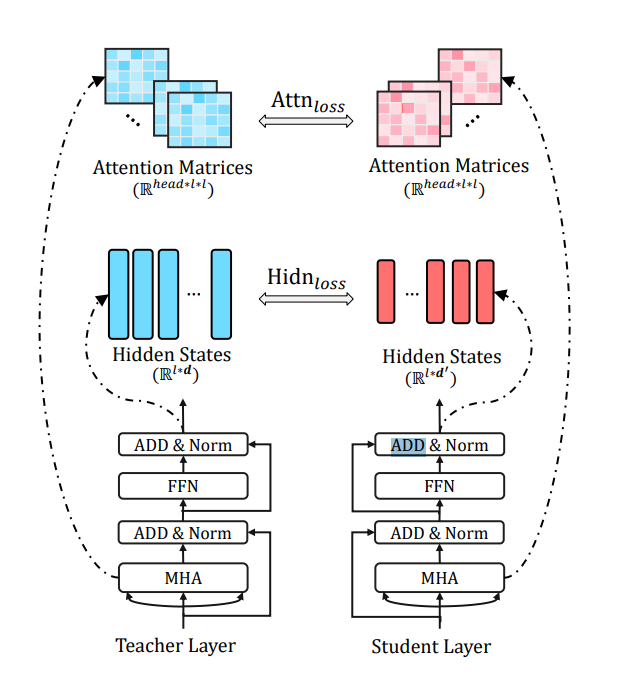
\includegraphics[width=0.5\textwidth]{Figs/MHA.png} 
	\caption{\small Dettagli del processo di distillazione a livello di strato del Transformer. La procedura integra la distillazione basata sull'attenzione ($Attn_{loss}$), calcolata sulle matrici di attenzione, e la distillazione basata sugli stati nascosti ($Hidn_{loss}$), applicata alle rappresentazioni latenti tra lo strato insegnante (\textit{Teacher Layer}) e lo strato studente (\textit{Student Layer}).}
	\label{fig:distillazione_transformer}
\end{figure}


Oltre ai moduli di attenzione, ogni blocco dell'architettura integra reti neurali di tipo \textit{feed-forward} che operano in modo indipendente su ciascuna posizione, garantendo una trasformazione non lineare delle rappresentazioni apprese. La stabilità dell'addestramento e la possibilità di stratificare decine di questi blocchi (dando vita a modelli estremamente profondi) sono assicurate dall'integrazione di connessioni residue (\textit{residual connections}) seguite da fasi di \textit{Layer Normalization}. Queste strutture permettono ai gradienti di fluire più agevolmente durante la retropropagazione, mitigando i rischi di degradazione del modello. In ultima analisi, la straordinaria efficacia del Transformer risiede proprio nella sua scalabilità e nell'efficienza computazionale derivante dalla parallelizzazione massiva, proprietà che hanno permesso di addestrare i moderni \textit{Large Language Models} su corpora di dimensioni globali, rendendo necessario, in fase di implementazione pratica, il ricorso a tecniche di ottimizzazione come la \textit{Knowledge Distillation} per bilanciare l'enorme complessità parametrica con le risorse hardware disponibili.
\end{comment}

\subsection{L'architettura Transformer}
\label{subsec:transformer}

L'introduzione dell'architettura \textbf{Transformer}, formalizzata da \citet{vaswani2017attention} attraverso il fondamentale articolo \textit{"Attention is All You Need"}, ha rappresentato un cambiamento di paradigma senza precedenti nel campo dell'elaborazione del linguaggio naturale (NLP). Prima della sua diffusione, lo stato dell'arte era dominato dalle reti neurali ricorrenti (RNN) e dalle loro varianti, come le \textit{Long Short-Term Memory} (LSTM) \cite{hochreiter1997long}, le quali elaboravano le sequenze di dati in modo intrinsecamente sequenziale. Tale approccio presentava due limitazioni critiche: la difficoltà nel gestire dipendenze a lungo raggio a causa del fenomeno della scomparsa del gradiente e l'impossibilità di parallelizzare efficacemente il calcolo, rendendo l'addestramento su grandi dataset estremamente oneroso in termini temporali. Il Transformer risolve radicalmente queste problematiche abbandonando la ricorsività a favore di un'architettura basata esclusivamente sul meccanismo di attenzione.

Il pilastro teorico e funzionale di questa architettura è rappresentato dal meccanismo di \textbf{Self-Attention} (auto-attenzione), un processo che permette al modello di esaminare ogni parola all'interno di una sequenza e determinare, attraverso un sistema di pesi dinamici, quali altri token siano più rilevanti per comprenderne il contesto, indipendentemente dalla loro distanza fisica nel testo. Da un punto di vista matematico, questa operazione si realizza proiettando ogni token di input in tre diversi spazi vettoriali, generando così tre matrici: la \textbf{Query} ($Q$), che rappresenta il token attuale in cerca di contesto; la \textbf{Key} ($K$), che contiene le informazioni salienti di tutti i token della sequenza; e il \textbf{Value} ($V$), che racchiude il contenuto informativo effettivo. L'interazione tra questi elementi avviene attraverso il calcolo del prodotto scalare tra Query e Key, il cui risultato viene normalizzato per determinare quanto peso assegnare a ciascun valore. La funzione di attenzione è definita formalmente come:

\begin{equation}
	\text{Attention}(Q, K, V) = \text{softmax}\left(\frac{QK^T}{\sqrt{d_k}}\right)V
\end{equation}

In questa espressione, il termine $\sqrt{d_k}$, dove $d_k$ è la dimensione delle chiavi, funge da fattore di scala cruciale per evitare che il prodotto scalare assuma valori eccessivamente elevati, i quali porterebbero la funzione softmax in regioni con gradienti estremamente piccoli, ostacolando l'apprendimento.



Per aumentare la capacità espressiva del modello, il Transformer non si limita a un singolo calcolo di attenzione, ma impiega la cosiddetta \textbf{Multi-Head Attention}. Questa tecnica consiste nell'eseguire molteplici operazioni di attenzione in parallelo, ognuna con i propri parametri lineari appresi; ciò consente al sistema di "osservare" la sequenza da diverse prospettive semantiche e sintattiche simultaneamente, catturando relazioni complesse che un unico meccanismo di attenzione non riuscirebbe a isolare. Tuttavia, la natura parallela del Transformer comporta la perdita intrinseca dell'informazione sull'ordine temporale delle parole, un elemento invece naturale nelle RNN. Per sopperire a questa mancanza, vengono introdotti i \textbf{Positional Encoding}, segnali sinusoidali di diversa frequenza che vengono sommati ai vettori di embedding iniziali. Tali segnali forniscono al modello una coordinata spaziale per ogni token, permettendogli di distinguere tra frasi con le stesse parole disposte in ordini differenti.


\begin{figure}[t]
	\centering
	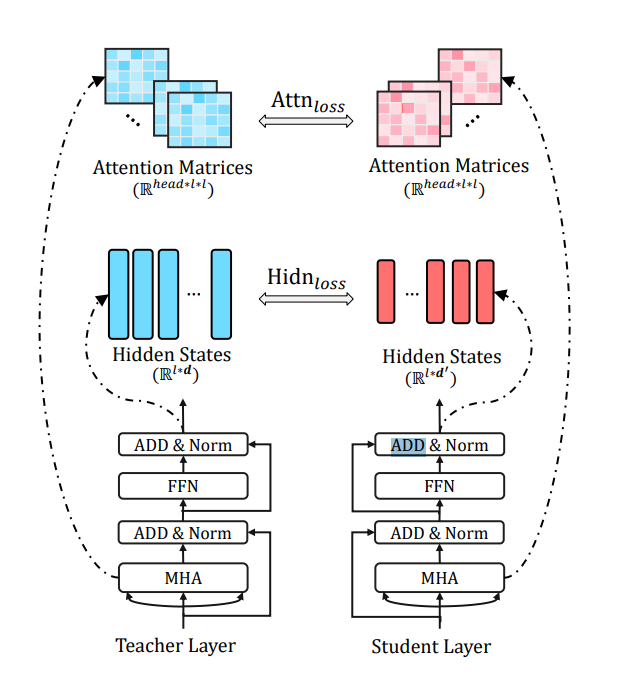
\includegraphics[width=0.5\textwidth]{Figs/MHA.png} 
	\caption{\small Dettagli del processo di distillazione a livello di strato del Transformer. La procedura integra la distillazione basata sull'attenzione ($Attn_{loss}$), calcolata sulle matrici di attenzione, e la distillazione basata sugli stati nascosti ($Hidn_{loss}$), applicata alle rappresentazioni latenti tra lo strato insegnante (\textit{Teacher Layer}) e lo strato studente (\textit{Student Layer}).}
	\label{fig:distillazione_transformer}
\end{figure}


Oltre ai moduli di attenzione, ogni blocco dell'architettura integra reti neurali di tipo \textit{feed-forward} che operano in modo indipendente su ciascuna posizione, garantendo una trasformazione non lineare delle rappresentazioni apprese. La stabilità dell'addestramento e la possibilità di stratificare decine di questi blocchi (dando vita a modelli estremamente profondi) sono assicurate dall'integrazione di connessioni residue (\textit{residual connections}) seguite da fasi di \textit{Layer Normalization}. Queste strutture permettono ai gradienti di fluire più agevolmente durante la retropropagazione, mitigando i rischi di degradazione del modello. In ultima analisi, la straordinaria efficacia del Transformer risiede proprio nella sua scalabilità e nell'efficienza computazionale derivante dalla parallelizzazione massiva, proprietà che hanno permesso di addestrare i moderni \textit{Large Language Models} su corpora di dimensioni globali, rendendo necessario, in fase di implementazione pratica, il ricorso a tecniche di ottimizzazione come la \textit{Knowledge Distillation} per bilanciare l'enorme complessità parametrica con le risorse hardware disponibili.

\subsection{Pre-training}

Il \textbf{Pre-training} costituisce la fase iniziale e computazionalmente più onerosa del ciclo di vita di un Large Language Model (LLM). In questa fase, il modello viene addestrato su una vastissima mole di dati non etichettati (\textit{unlabelled data}) provenienti da fonti eterogenee quali il web (ad esempio Common Crawl), libri, articoli scientifici, documentazione tecnica e codice sorgente. Con il termine \textbf{unlabelled data} si fa riferimento a informazioni grezze prive di una \textit{ground truth} definita a priori; il modello, pertanto, non riceve istruzioni esplicite sul significato dei dati da parte di un supervisore umano, ma è chiamato a inferirne autonomamente le regolarità statistiche e le strutture latenti.
L'obiettivo primario del pre-training è l'apprendimento \textbf{self-supervised learning} (\textit{self-supervised learning}), generalmente implementato attraverso il task di \textit{Next Token Prediction}. In questo contesto, dato un contesto testuale parziale, il modello deve stimare la distribuzione di probabilità del token successivo, aggiornando i propri parametri in modo da minimizzare una funzione di perdita, tipicamente la \textit{cross-entropy loss}. Sebbene il compito appaia semplice, la sua ripetizione su miliardi o trilioni di esempi consente al modello di apprendere relazioni sintattiche, strutture grammaticali complesse, dipendenze semantiche a lungo raggio e, in maniera implicita, una vasta conoscenza enciclopedica del mondo.
Un aspetto cruciale del pre-training riguarda la \textbf{preparazione e la curazione dei dati}. Prima dell’addestramento, i dataset vengono sottoposti a processi di filtraggio, deduplicazione e normalizzazione al fine di ridurre il rumore, eliminare contenuti ridondanti e migliorare la qualità complessiva delle informazioni. Successivamente, il testo viene trasformato in una sequenza di token tramite tecniche di \textbf{tokenizzazione} (come Byte Pair Encoding o Unigram Language Model), che consentono di rappresentare il linguaggio naturale in una forma numerica trattabile dalle reti neurali.
Dal punto di vista computazionale, il pre-training richiede infrastrutture hardware altamente specializzate, basate su GPU o TPU, e strategie di ottimizzazione avanzate come il \textit{data parallelism} e il \textit{model parallelism}. La letteratura ha inoltre evidenziato l’esistenza di \textbf{scaling laws}, secondo cui le prestazioni del modello migliorano in modo prevedibile all’aumentare della quantità di dati, del numero di parametri e delle risorse computazionali impiegate. Tuttavia, tali benefici sono accompagnati da costi energetici ed economici significativi, rendendo il pre-training una fase accessibile solo a pochi attori industriali e accademici dotati di risorse adeguate.
Il risultato finale del pre-training è il cosiddetto \textbf{Base Model}: un modello generale, capace di generare testo coerente e plausibile su una vasta gamma di argomenti, ma privo di un allineamento esplicito a obiettivi specifici, preferenze umane o vincoli etici. In questa fase, il comportamento del modello riflette unicamente le distribuzioni statistiche apprese dai dati di addestramento. Per tale motivo, il pre-training rappresenta una base necessaria ma non sufficiente: esso fornisce le fondamenta cognitive del sistema, che verranno successivamente raffinate attraverso fasi di \textit{fine-tuning} e \textit{alignment}, finalizzate a rendere il modello più utile, sicuro e aderente ai contesti applicativi desiderati.


\subsection{Fine-tuning}

Mentre il pre-training fornisce al modello una conoscenza generale e trasversale, il \textbf{Fine-tuning} rappresenta la fase di adattamento (\textit{transfer learning}) del sistema a un dominio applicativo specifico o a un compito ben definito. In questa fase, il \textit{Base Model} viene ulteriormente addestrato su un dataset più contenuto ma altamente specializzato, composto da dati supervisionati (\textit{labelled data}), con l’obiettivo di orientarne il comportamento verso prestazioni elevate in contesti mirati.

\begin{figure}[t]
    \centering
    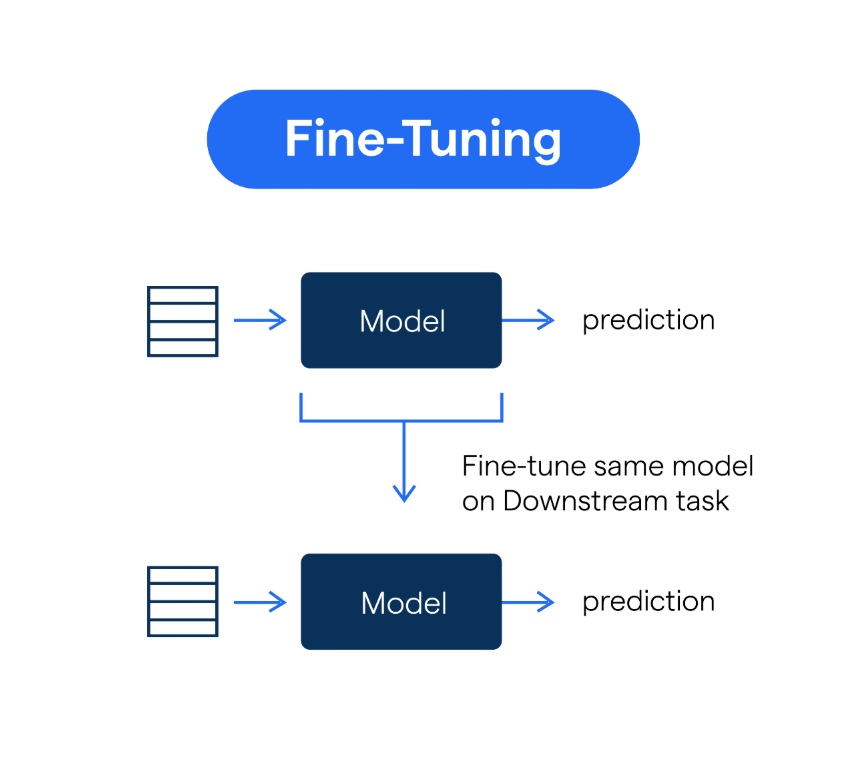
\includegraphics[width=0.8\textwidth]{Figs/fine tuning.png} 
    \caption[Schema del processo di Fine-Tuning]{\small \textbf{Schema del processo di Fine-Tuning.} L'illustrazione mostra la transizione di un modello linguistico da una configurazione generica a una specializzata. Partendo da un modello pre-addestrato che genera predizioni standard, il processo prevede un ulteriore addestramento su un dataset specifico (\textit{downstream task}) per ottimizzare i parametri e adattare il comportamento del sistema a compiti o domini verticali mirati.}
    \label{fig:fine_tuning_schema}
\end{figure}

A differenza del pre-training, il fine-tuning si fonda sull’impiego di dati \textbf{etichettati}: a ogni input è associata un’annotazione esplicita, fornita da un agente esterno — tipicamente un annotatore umano o un sistema automatico di labeling — che rappresenta la risposta corretta o la classe di appartenenza del dato. Tali etichette fungono da segnale di apprendimento diretto, consentendo al modello di aggiornare i propri parametri in modo guidato e di ridurre l’ambiguità interpretativa tipica dei modelli generalisti.

Dal punto di vista metodologico, il fine-tuning può assumere forme differenti a seconda del compito da svolgere. Nei problemi di classificazione, ad esempio, il modello viene ottimizzato per associare correttamente un input a una categoria predefinita; nei compiti di \textit{question answering} o di generazione controllata del testo, l’obiettivo è invece massimizzare la coerenza e la correttezza delle risposte rispetto alle annotazioni fornite. In tutti i casi, la funzione di perdita è progettata per penalizzare le discrepanze tra l’output del modello e le etichette di riferimento, rafforzando progressivamente i comportamenti desiderati.

L’importanza del fine-tuning risiede nella sua capacità di \textbf{specializzare} il modello senza dover ripetere l’intero processo di pre-training. Un LLM generico può così essere adattato a domini verticali quali l’ambito legale, medico, finanziario o ingegneristico, acquisendo familiarità con il linguaggio tecnico, le convenzioni formali e le tipologie di problemi caratteristiche di ciascun settore. Questo approccio consente di ottenere modelli altamente performanti anche in presenza di dataset relativamente piccoli, sfruttando la conoscenza latente già appresa nella fase precedente.

Tuttavia, il fine-tuning tradizionale presenta alcune criticità. Una delle più rilevanti è il fenomeno del \textit{catastrophic forgetting}, ovvero la tendenza del modello a perdere parte delle competenze generali acquisite durante il pre-training quando viene ottimizzato in modo intensivo su un dominio ristretto. Inoltre, l’aggiornamento di tutti i parametri di un LLM comporta un costo computazionale elevato e richiede significative risorse hardware, rendendo il processo poco scalabile in molti contesti applicativi.

Per affrontare tali limitazioni, negli ultimi anni sono state sviluppate tecniche di \textbf{Parameter-Efficient Fine-Tuning} (PEFT), tra cui spicca LoRA (\textit{Low-Rank Adaptation}) \cite{hu2021lora}. Questi approcci mirano a congelare la maggior parte dei parametri del modello di base e ad addestrare solo un sottoinsieme ridotto di pesi aggiuntivi, spesso organizzati in matrici a rango ridotto. Lavori precedenti avevano esplorato direzioni analoghe tramite adapter layers \cite{houlsby2019parameter}, prefix tuning \cite{li2021prefix} e prompt tuning \cite{lester2021power}. In questo modo, è possibile adattare il modello a nuovi compiti riducendo drasticamente il consumo di memoria, il tempo di addestramento e il rischio di perdita delle capacità generali.

Il fine-tuning rappresenta un passaggio fondamentale per trasformare un modello linguistico generico in uno strumento realmente utile in contesti applicativi concreti. Esso funge da ponte tra la conoscenza generale appresa durante il pre-training e le esigenze specifiche del mondo reale, ponendo le basi per ulteriori fasi di ottimizzazione e allineamento orientate all’interazione efficace e affidabile con l’utente finale.


\begin{comment}
\subsection{Instruction Tuning}

L'\textbf{Instruction Tuning} rappresenta una forma evoluta di fine-tuning, fondamentale per rendere i modelli realmente utilizzabili dagli utenti finali sotto forma di assistenti digitali. Senza questa fase, un modello pre-addestrato tenderebbe a "completare" un comando piuttosto che a "eseguirlo" (ad esempio, davanti alla domanda "Qual è la capitale della Francia?", un base model potrebbe rispondere continuando la lista con "Qual è la capitale della Germania?").

Attraverso l'Instruction Tuning, il modello viene esposto a dataset composti da coppie di \textbf{istruzione-risposta}. Questo processo insegna al modello a interpretare l'intento dell'utente e a conformarsi a uno specifico formato di output. Questa tecnica è spesso il prerequisito per fasi successive di allineamento, come il \textit{Reinforcement Learning from Human Feedback} (RLHF). 

\begin{figure}[htbp]
    \centering
    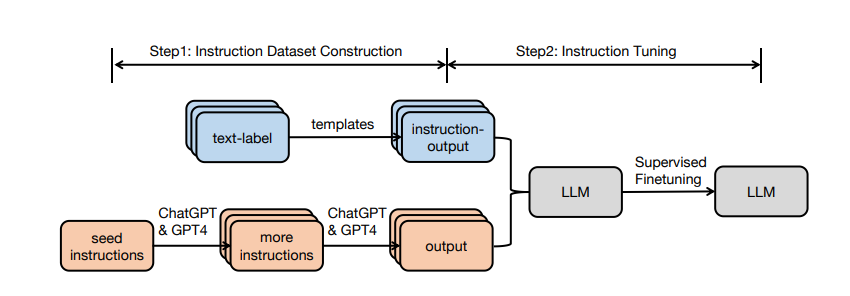
\includegraphics[width=0.8\textwidth]{Figs/pipeline generica di instruction tuning.png}
    \caption{\small Panoramica della pipeline di \textit{Instruction Tuning}.}
    \label{fig:instruction_tuning_pipeline}
\end{figure}

L'\textbf{Instruction Tuning} e la \textbf{Knowledge distillation} sono collegati, siccome molti approcci di Instruction Tuning si basano sulla distillation di modelli di grandi dimensioni, utilizzati come teacher per generare dati di addestramento di alta qualità destinati a modelli più piccoli e più efficienti.

La \textbf{Knowledge Distillation} esercita un'influenza significativa sull'Instruction Tuning, poiché non solo permette di trasferire la conoscenza di un modello ma anche la capacità di ragionamento e di strutturazione delle risposte da un modello \textit{teacher} a uno \textit{student}. In questo contesto, il modello di grandi dimensioni, spesso già allineato tramite Instruction Tuning o RLHF, viene impiegato per generare risposte di alta qualità a un ampio insieme di istruzioni, crando un dataset sintetico che guida l'addestramento di modelli più piccoli ed efficienti.

Molti approcci moderni di \textbf{Instruction Tuning} possono essere interpretati come una forma implicita di distillation, in cui il comportamento desiderato del modello non è appreso direttamente da annotazioni umane, ma viene approssimato replicando le risposte e i pattern decisionali di un modello più performante.

L'influenza della distillation sull'Instruction Tuning risulta particolarmente importante anche sul piano pratico. L'utilizzo di dati generati da modelli \textit{teacher} consente di ridurre significativamente i costi di raccolta di dataset annotati manualmente, migliorando al contempo la qualità e la coerenza delle risposte apprese. Inoltre, tale approccio favorisce la scalabilità del processo di allineamento, rendendo possibile l'addestramento di modelli instruction-tuned destinati a operare su dispositivi o architetture con risorse computazionali limitate.

\end{comment}

\subsection{Instruction Tuning}

L'\textbf{Instruction Tuning} rappresenta una forma evoluta di fine-tuning, fondamentale per rendere i modelli realmente utilizzabili dagli utenti finali sotto forma di assistenti digitali. Senza questa fase, un modello pre-addestrato tenderebbe a ``completare'' un comando piuttosto che a ``eseguirlo'' (ad esempio, davanti alla domanda ``Qual è la capitale della Francia?'', un base model potrebbe rispondere continuando la lista con ``Qual è la capitale della Germania?''). Attraverso l'Instruction Tuning \cite{wei2022finetuned,wang2022self}, il modello viene esposto a dataset composti da coppie di \textbf{istruzione-risposta}: come mostrato in Figura~\ref{fig:instruction_tuning_pipeline}, la pipeline prevede tipicamente la raccolta di istruzioni eterogenee, la generazione delle risposte corrispondenti e il successivo fine-tuning del modello base su questo insieme strutturato. Questo processo insegna al modello a interpretare l'intento dell'utente e a conformarsi a uno specifico formato di output, ed è spesso il prerequisito per fasi successive di allineamento, come il \textit{Reinforcement Learning from Human Feedback} (RLHF) \cite{ouyang2022training}.

L'\textbf{Instruction Tuning} e la \textbf{Knowledge Distillation} sono strettamente collegati: molti approcci moderni si basano sulla distillazione di modelli di grandi dimensioni, utilizzati come \textit{teacher} per generare dati di addestramento di alta qualità destinati a modelli più piccoli ed efficienti. La Knowledge Distillation non permette infatti di trasferire solo la conoscenza fattuale, ma anche la capacità di ragionamento e di strutturazione delle risposte. In questo contesto, il modello \textit{teacher} — spesso già allineato tramite Instruction Tuning o RLHF — viene impiegato per generare risposte ad un ampio insieme di istruzioni, creando un dataset sintetico che guida l'addestramento dello \textit{student}. Molti approcci moderni di Instruction Tuning possono pertanto essere interpretati come una forma implicita di distillazione, in cui il comportamento desiderato non è appreso direttamente da annotazioni umane, ma viene approssimato replicando i pattern decisionali del modello più performante.

Questa sinergia risulta rilevante anche sul piano pratico: l'utilizzo di dati generati dal \textit{teacher} consente di ridurre significativamente i costi di raccolta di dataset annotati manualmente, migliorando al contempo la qualità e la coerenza delle risposte apprese. Inoltre, tale approccio favorisce la scalabilità del processo di allineamento, rendendo possibile l'addestramento di modelli instruction-tuned destinati a operare su dispositivi o architetture con risorse computazionali limitate.

\begin{figure}[t]
    \centering
    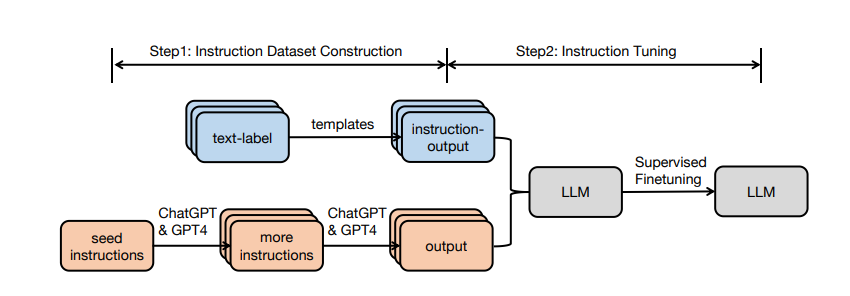
\includegraphics[width=0.8\textwidth]{Figs/pipeline generica di instruction tuning.png}
    \caption{Panoramica della pipeline di \textit{Instruction Tuning}.}
    \label{fig:instruction_tuning_pipeline}
\end{figure}

\section{Knowledge Distillation}

La \textbf{Knowledge Distillation} (KD) rappresenta una delle tecniche più efficaci per la compressione dei modelli, permettendo di trasferire le capacità di un'architettura vasta e complessa (\textbf{Teacher}) a una più compatta ed efficiente (\textbf{Student}). La KD non si basa esclusivamente sull'apprendimento da dati etichettati, ma introduce un cambio di paradigma basato sulla qualità dell'informazione trasmessa.

Il successo di questa tecnica risiede nel superamento del concetto di "etichetta rigida" (\textit{hard target}) tipico del fine-tuning classico. Mentre in un dataset standard ogni esempio è associato a una verità univoca (dove la classe corretta ha probabilità 1 e le altre 0), la distillazione attinge alla cosiddetta \textbf{Dark Knowledge}. Come teorizzato da \citet{hinton2015distilling}, questa "conoscenza oscura" è racchiusa nelle distribuzioni di probabilità prodotte dal modello Teacher, i cosiddetti \textbf{soft targets}. 


\begin{figure}[t]
    \centering
    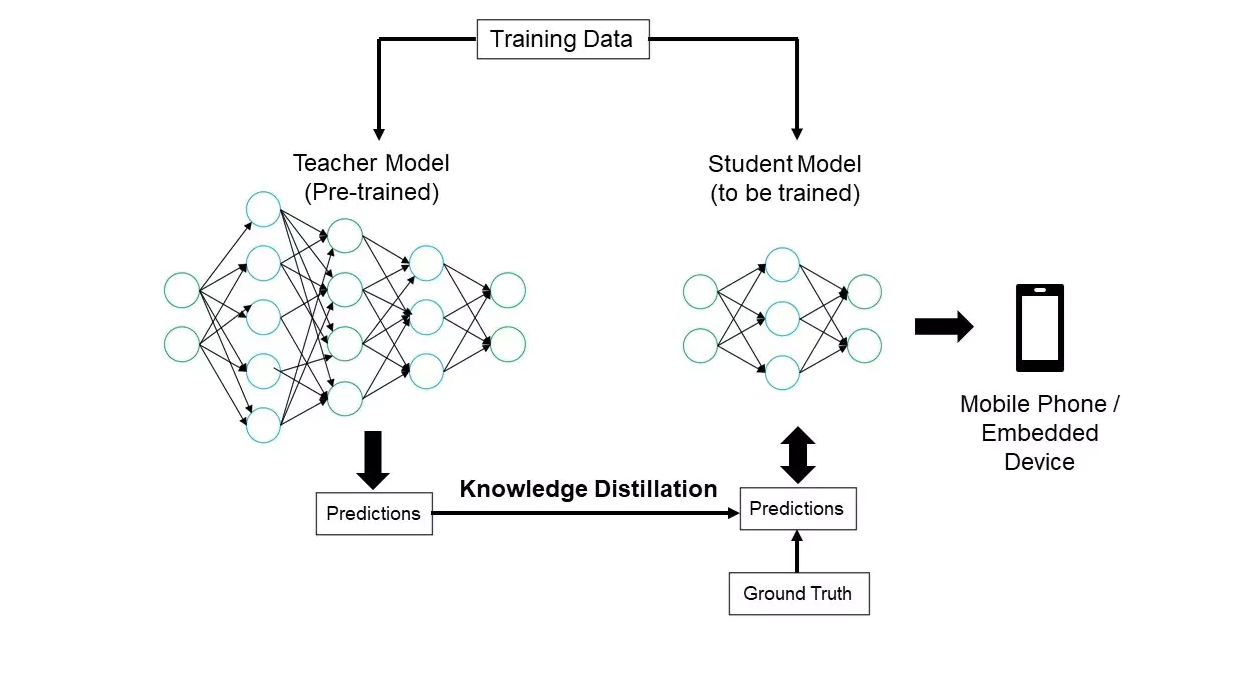
\includegraphics[width=0.8\textwidth]{Figs/distillation.png} 
    \caption[Schema del processo di Knowledge Distillation]{\small \textbf{Rappresentazione del processo di Knowledge Distillation.} Il framework illustra il trasferimento di conoscenza da un \textit{Teacher Model} (pre-addestrato e di grandi dimensioni) a uno \textit{Student Model} più compatto. Attraverso il confronto delle predizioni e l'integrazione con la \textit{Ground Truth}, lo studente viene ottimizzato per operare su dispositivi con risorse limitate, come smartphone o sistemi embedded, mantenendo prestazioni paragonabili al modello più complesso.}
    \label{fig:knowledge_distillation}
\end{figure}


Analizzando i soft targets, lo studente non impara solo qual è la risposta corretta, ma apprende le relazioni semantiche tra le classi. Ad esempio, se il Teacher assegna una probabilità residua più alta alla classe "cane" rispetto alla classe "gatto" mentre analizza l'immagine di un lupo, sta comunicando allo studente una gerarchia di somiglianza che un'etichetta binaria ometterebbe. Per estrarre efficacemente questa conoscenza, viene applicato un parametro di \textbf{Temperatura} ($T$) alla funzione \textit{softmax}:

\begin{equation}
    P_i = \frac{\exp(z_i / T)}{\sum_{j} \exp(z_j / T)}
\end{equation}

L'innalzamento della temperatura ($T > 1$) durante la fase di training permette di "ammorbidire" la distribuzione di probabilità, rendendo più evidenti le sfumature decisionali del Teacher. In questo modo, lo Student può emulare il comportamento logico del modello più grande, raggiungendo prestazioni comparabili pur operando con una frazione dei parametri e delle risorse computazionali. La Knowledge Distillation si configura quindi non solo come uno strumento di efficienza, ma come un processo di raffinamento qualitativo del sapere appreso.

\subsection{Definizione e principi fondamentali}

La \textbf{Knowledge Distillation} (KD) va ben oltre la semplice compressione di un modello riducendone i parametri. È piuttosto un processo elegante e sofisticato che permette di trasferire l’«intelligenza» statistica accumulata da un modello grande (il teacher) a uno più piccolo e leggero (lo student). In pratica, non ci limitiamo a rendere il modello più veloce o meno costoso: cerchiamo di fargli «capire» e ragionare in modo simile a come lo fa il modello più capace, imparando non solo le risposte corrette, ma anche il modo in cui il teacher arriva a quelle risposte. Il principio cardine, formalizzato da \citet{hinton2015distilling}, risiede nell'osservazione che il comportamento di un modello complesso (\textit{Teacher}) contiene informazioni molto più ricche rispetto alle semplici etichette binarie presenti nei dataset tradizionali. Mentre il fine-tuning classico minimizza l'errore rispetto a una \textit{ground truth} rigida (dove una sola classe è corretta e le altre sono considerate parimenti errate), la KD sfrutta la \textbf{Dark Knowledge}.

Questa "conoscenza oscura" è codificata nelle probabilità relative che il \textit{Teacher} assegna alle classi errate. Se, in un compito di classificazione testuale, il \textit{Teacher} assegna una probabilità dello $0.1\%$ alla categoria "sport" e dello $0.0001\%$ alla categoria "cucina" per un testo che parla di "salute", sta comunicando allo \textit{Student} che l'argomento salute è semanticamente più vicino allo sport che alla cucina. Questo segnale di supervisione supplementare permette allo \textit{Student} di apprendere la geometria dello spazio latente del \textit{Teacher}, portando a una generalizzazione superiore.

Dal punto di vista matematico, l'efficacia del trasferimento è regolata dalla funzione di \textbf{Loss di Distillazione}. Lo \textit{Student} viene addestrato minimizzando una funzione di costo composta:
\begin{equation}
    \mathcal{L} = (1 - \alpha) \mathcal{L}_{CE}(y, \sigma(z_s)) + \alpha T^2 \mathcal{L}_{KL}(\sigma(z_t/T), \sigma(z_s/T))
\end{equation}
dove $\mathcal{L}_{CE}$ è la \textit{cross-entropy} standard rispetto alle etichette reali $y$, mentre $\mathcal{L}_{KL}$ è la divergenza di Kullback-Leibler tra le distribuzioni del docente ($z_t$) e dello studente ($z_s$). Il parametro $\alpha$ bilancia l'importanza dei due segnali, mentre la temperatura $T$ gioca un ruolo cruciale: all'aumentare di $T$, la distribuzione dei \textit{logits} si appiattisce, forzando lo \textit{Student} a prestare attenzione non solo al picco di probabilità, ma anche alle relazioni di somiglianza tra le classi meno probabili.

\subsection{Paradigma Teacher--Student}

Il paradigma \textbf{Teacher--Student} non rappresenta soltanto una tecnica di compressione, ma definisce una vera e propria relazione pedagogica tra architetture neurali con obiettivi divergenti. Il \textbf{Teacher} si configura tipicamente come un modello sovra-parametrizzato, come GPT-4 \cite{achiam2023gpt4} o LLaMA \cite{touvron2023llama}, che ha raggiunto la saturazione prestazionale durante il pre-training grazie a centinaia di miliardi di parametri. Sebbene tale complessità garantisca una straordinaria capacità di generalizzazione, essa si traduce in un'inefficienza computazionale critica in termini di latenza e occupazione di memoria VRAM, rendendo il modello difficilmente utilizzabile in scenari \textit{edge} o in tempo reale.

In questo contesto, lo \textbf{Student} emerge come un'architettura snella progettata per operare entro vincoli hardware stringenti, come illustrato in Figura~\ref{fig:teacher_student_architecture}. La sua genesi può seguire percorsi differenti: da un lato la \textit{riduzione strutturale}, in cui lo Student eredita la topologia del Teacher riducendo però il numero di layer, le teste di attenzione o la dimensione degli embedding; dall'altro, l'adozione di \textit{architetture eterogenee}, dove la conoscenza viene trasposta in modelli ottimizzati per specifici processori, come il passaggio da un trasformatore massivo a una rete convoluzionale o a una ricorrente (RNN) più agile.

Un elemento di criticità in questa transizione è rappresentato dal \textbf{Capacity Gap}. Qualora il divario tra le capacità dei due modelli sia eccessivo, lo Student può fallire nell'imitazione poiché le funzioni decisionali del Teacher risultano troppo complesse per essere approssimate da un numero limitato di parametri. Per mitigare questo fenomeno, la letteratura suggerisce l'impiego della \textit{Multi-stage Distillation} o l'introduzione di un \textit{Teacher Assistant} \cite{mirzadeh2020improved}: un modello di taglia intermedia che funge da ponte cognitivo, facilitando un trasferimento graduale della conoscenza e riducendo la perdita di accuratezza finale.

\begin{figure}[t]
    \centering
    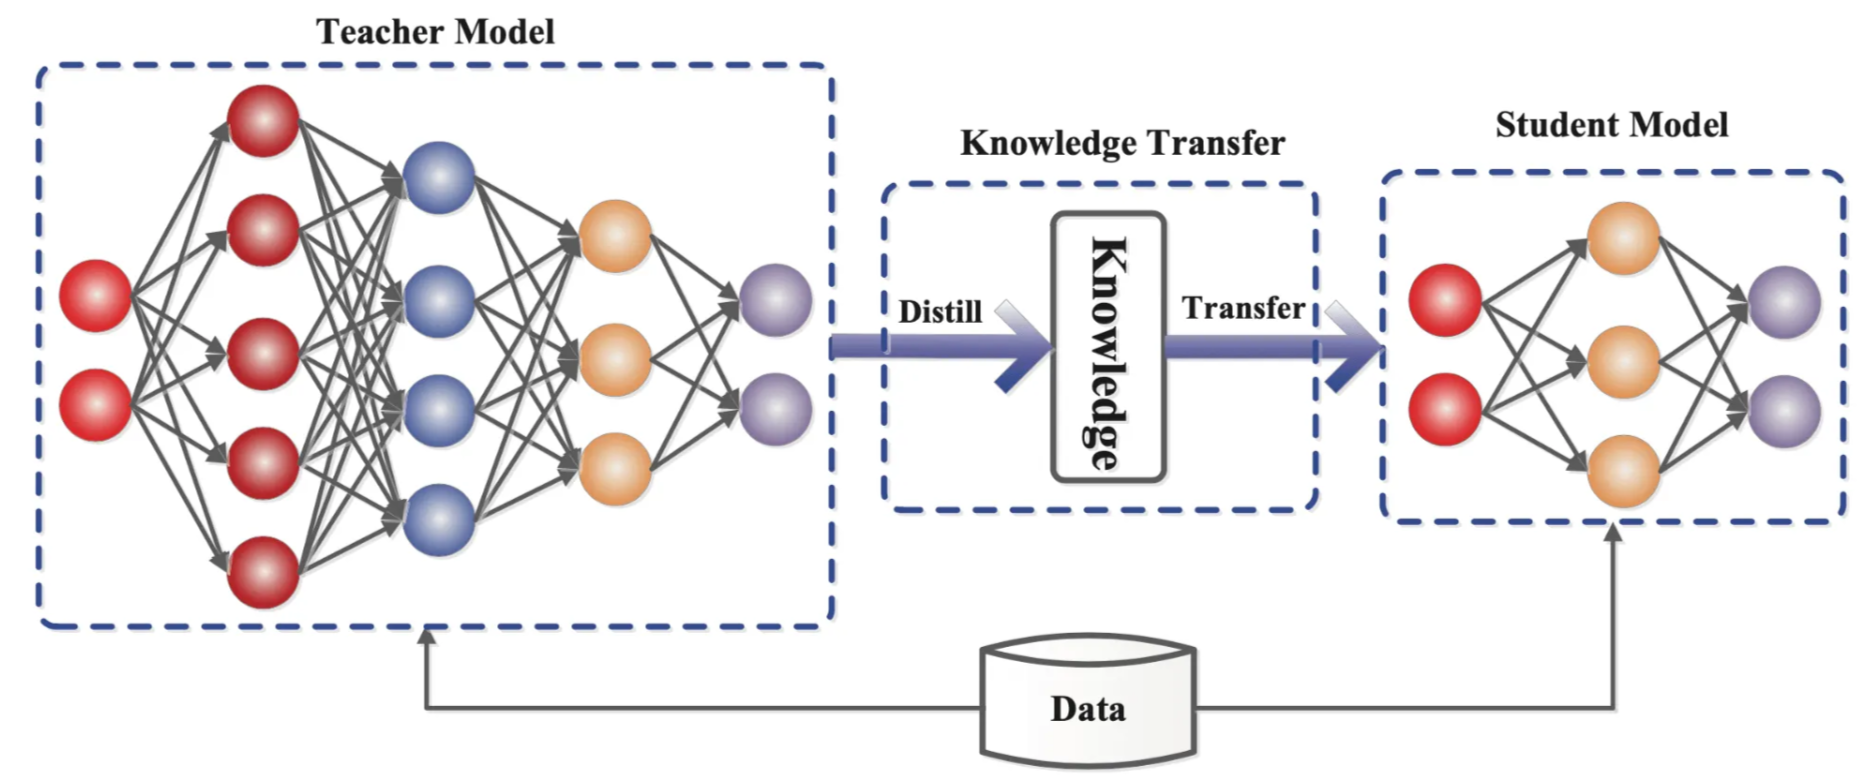
\includegraphics[width=0.8\textwidth]{Figs/teacher-student.png}
    \caption{Architettura di trasferimento della conoscenza da un modello \textit{Teacher} a uno \textit{Student} di dimensioni ridotte.}
    \label{fig:teacher_student_architecture}
\end{figure}

\subsection{Modalità di trasferimento della conoscenza}

Il trasferimento della conoscenza può essere declinato attraverso diverse metodologie operative che variano in base al livello di introspezione richiesto sul modello docente. La forma più accessibile è la \textbf{Response-based Distillation}, comunemente nota come \textit{Logits Distillation}. In questo scenario, lo Student si focalizza esclusivamente sull'output finale, cercando di replicare le distribuzioni di probabilità prodotte dal Teacher. Tale approccio è particolarmente vantaggioso quando si opera con modelli proprietari accessibili solo tramite API, poiché non richiede l'accesso ai pesi interni o alle attivazioni del sistema sorgente. Tuttavia, questa modalità è anche la più superficiale: cattura solo il comportamento esterno del modello senza comprendere i meccanismi interni che hanno portato a quella decisione.

Andando più in profondità, la \textbf{Feature-based Distillation} (o \textit{Hint Training}) \cite{romero2015fitnets} mira ad allineare le rappresentazioni intermedie dei due modelli. Poiché i layer interni catturano astrazioni semantiche e sintattiche fondamentali, lo Student viene forzato a produrre attivazioni simili a quelle del docente in strati specifici della rete. 

\begin{figure}[t]
    \centering
    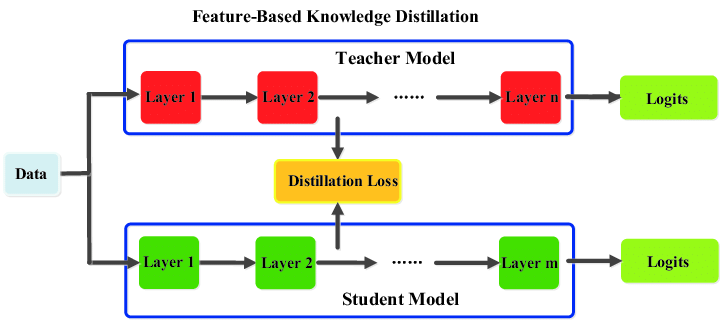
\includegraphics[width=0.8\textwidth]{Figs/The-generic-feature-based-knowledge-distillation.png}
    \caption{\small Architettura concettuale della \textit{Feature-Based Knowledge Distillation}. Il processo prevede il trasferimento di conoscenza attraverso l'allineamento delle mappe di caratteristiche intermedie (feature maps) prodotte dai livelli interni del modello \textit{Teacher} e del modello \textit{Student}. La \textit{Distillation Loss} viene calcolata per minimizzare la discrepanza tra le rappresentazioni latenti dei due modelli durante la fase di addestramento.}
    \label{fig:feature_based_kd}
\end{figure}

Questo approccio permette di trasmettere non solo il \textit{cosa} (l'output finale), ma anche il \textit{come} — ovvero la struttura gerarchica con cui l'informazione viene elaborata. Data la frequente discrepanza dimensionale tra i layer dei due modelli — ad esempio tra un Teacher da 4096 neuroni e uno Student da 768 — si ricorre all'uso di \textit{regressor layer} o proiezioni lineari che mappano lo spazio latente dello Student in quello del Teacher, permettendo un confronto diretto tra le mappe di caratteristiche. Sebbene più efficace della semplice imitazione degli output, questa tecnica richiede accesso completo all'architettura del Teacher e comporta un costo computazionale maggiore durante l'addestramento.

Un'ulteriore evoluzione è rappresentata dalla \textbf{Relation-based Distillation} \cite{park2019relational}, che sposta l'attenzione dai singoli punti dati alle relazioni intercorrenti tra essi. 
Invece di imitare una singola risposta o una singola attivazione, lo Student apprende come il Teacher correla diversi esempi all'interno di un batch o come struttura l'attenzione tra i token in una sequenza. Attraverso l'estrazione di matrici di similarità o mappe di \textit{Self-Attention}, lo Student acquisisce la capacità di pesare l'importanza dei contesti in modo analogo al docente. Questa modalità si rivela particolarmente efficace nei modelli Transformer, dove il meccanismo di attenzione codifica esplicitamente le dipendenze strutturali tra le parole, consentendo allo studente di ereditare pattern di ragionamento relazionale complessi che emergono solo dall'interazione tra più esempi.

\begin{figure}[htbp]
    \centering
    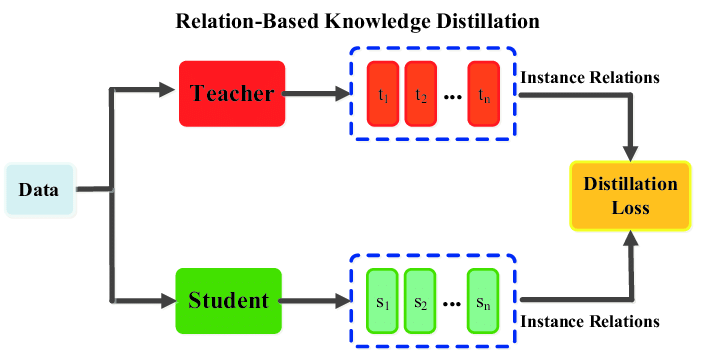
\includegraphics[width=0.8\textwidth]{Figs/The-generic-instance-relation-based-knowledge-distillation.png}
    \caption{\small Schema generale del processo di \textit{Relation-Based Knowledge Distillation}. Il dataset viene processato parallelamente dal modello Teacher e dal modello Student. La distillazione avviene minimizzando la discrepanza tra le relazioni inter-istanza (distanze o similarità tra i campioni $t_n$ e $s_n$) apprese dai due modelli.}
    \label{fig:feature_distillation}
\end{figure}

Infine, con l'avvento dei modelli di ragionamento avanzato come GPT-4 e i sistemi della famiglia o1, si è imposta la \textbf{Logic and Reasoning Distillation} \cite{hsieh2023distilling}. In questa modalità, il trasferimento riguarda le cosiddette \textit{Chain of Thought} (catene di pensiero) \cite{wei2022chain}: lo Student non apprende solo la risposta corretta, ma viene addestrato a replicare i passaggi logici intermedi — le argomentazioni, le verifiche e i ragionamenti controfattuali — che il Teacher esplicita prima di giungere alla conclusione finale. Questo approccio acquisisce capacità di \textit{problem-solving} strutturato che trascendono la mera distribuzione statistica dei token, avvicinando il modello compresso a una forma di ragionamento simbolico implicito.

Va sottolineato che queste strategie non sono mutuamente esclusive. Molti lavori recenti combinano più livelli di distillazione simultaneamente: si può, ad esempio, applicare una perdita sui logits finali insieme a una perdita sulle rappresentazioni intermedie e sulle matrici di attenzione, pesando opportunamente i diversi contributi nella funzione obiettivo complessiva. La scelta della strategia dipende da un trade-off tra accessibilità del Teacher, complessità computazionale dell'addestramento e fedeltà del trasferimento desiderata. L'integrazione sinergica di queste tecniche trasforma la Knowledge Distillation in un pilastro fondamentale per la democratizzazione dell'intelligenza artificiale, permettendo di distribuire capacità di ragionamento sofisticate su dispositivi di consumo quotidiano.

\section{Reflection Tuning}

Il \textbf{Reflection Tuning} \cite{ze2023reflection} rappresenta un'evoluzione paradigmatica nel campo dell'addestramento dei Large Language Models (LLM), spostando il focus dalla mera generazione di testo alla strutturazione del pensiero critico. Mentre l'approccio standard all'Instruction Tuning si limita a ottimizzare il modello affinché produca risposte conformi a un dato input, il Reflection Tuning mira a internalizzare un processo di supervisione cognitiva. Tale metodologia affronta uno dei limiti intrinseci dei modelli basati su Transformer: la natura "unidirezionale" e immediata del campionamento dei token, che spesso porta a errori logici dovuti alla mancanza di una fase di pianificazione o revisione interna.

\subsection{Concetto di self-reflection nei modelli linguistici}

Il concetto di \textbf{self-reflection} nell'ambito dell'intelligenza artificiale non rappresenta una semplice espansione algoritmica, ma un cambio di paradigma che si ispira direttamente alle capacità metacognitive umane. Tale processo definisce la facoltà del modello di monitorare, valutare e regolare i propri processi di pensiero in tempo reale. Nei modelli linguistici tradizionali, l'inferenza avviene solitamente in modo ``greedy'' o stocastico, dove ogni token viene generato in una sequenza lineare senza possibilità di revisione. La riflessione rompe questa linearità introducendo una pausa computazionale strategica: il modello esamina le proprie premesse e valuta la coerenza delle proprie deduzioni prima di cristallizzarle in un output definitivo.

Dal punto di vista della psicologia cognitiva, questo approccio implementa il cosiddetto \textbf{Dual Process Theory} proposto da \citet{kahneman2011thinking}. Mentre i modelli standard operano principalmente in modalità \textit{Sistema 1} — caratterizzata da una risposta veloce, istintiva e basata su pattern statistici immediati — la self-reflection abilita il \textit{Sistema 2}. Quest'ultimo è lento, deliberativo e analitico, e permette al modello di allocare una quota maggiore di risorse computazionali, definita \textit{Inference-time Compute}, per risolvere ambiguità semantiche o complessità logiche che richiederebbero una visione d'insieme superiore a quella offerta dalla semplice previsione del token successivo.

Tecnicamente, la riflessione si realizza attraverso la generazione di una ``traccia di pensiero'' (\textit{reasoning trace}) che funge da memoria di lavoro dinamica. Come illustrato in Figura~\ref{fig:riflection_tuning}, il processo di Reflection Tuning articola l'interazione tra \textit{Teacher} e \textit{Student Model} in tre fasi sequenziali: una prima fase di riflessione selettiva sulle istruzioni, una seconda di riflessione selettiva sulla risposta, e una terza di Instruction Tuning finale sul dataset curato. Durante ciascuna di queste fasi, il modello opera una scomposizione del task, suddividendo istruzioni articolate in sotto-obiettivi atomici affrontati sequenzialmente, filtrando i dati in base a difficoltà e fattibilità. Questo meccanismo permette di verificare la coerenza interna, controllando se i passaggi intermedi contraddicano i dati forniti nel prompt o la conoscenza pregressa memorizzata nei pesi sinaptici. Inoltre, il modello può simulare diverse traiettorie di risposta, valutando virtualmente quale percorso conduca alla probabilità logica più elevata prima di impegnarsi nella scrittura. Tale processo riduce drasticamente le cosiddette \textbf{allucinazioni di ragionamento}, poiché la risposta finale non emerge dal nulla, ma poggia su una catena logica precedentemente validata e corretta dal modello stesso.

\begin{figure}[t]
    \centering
    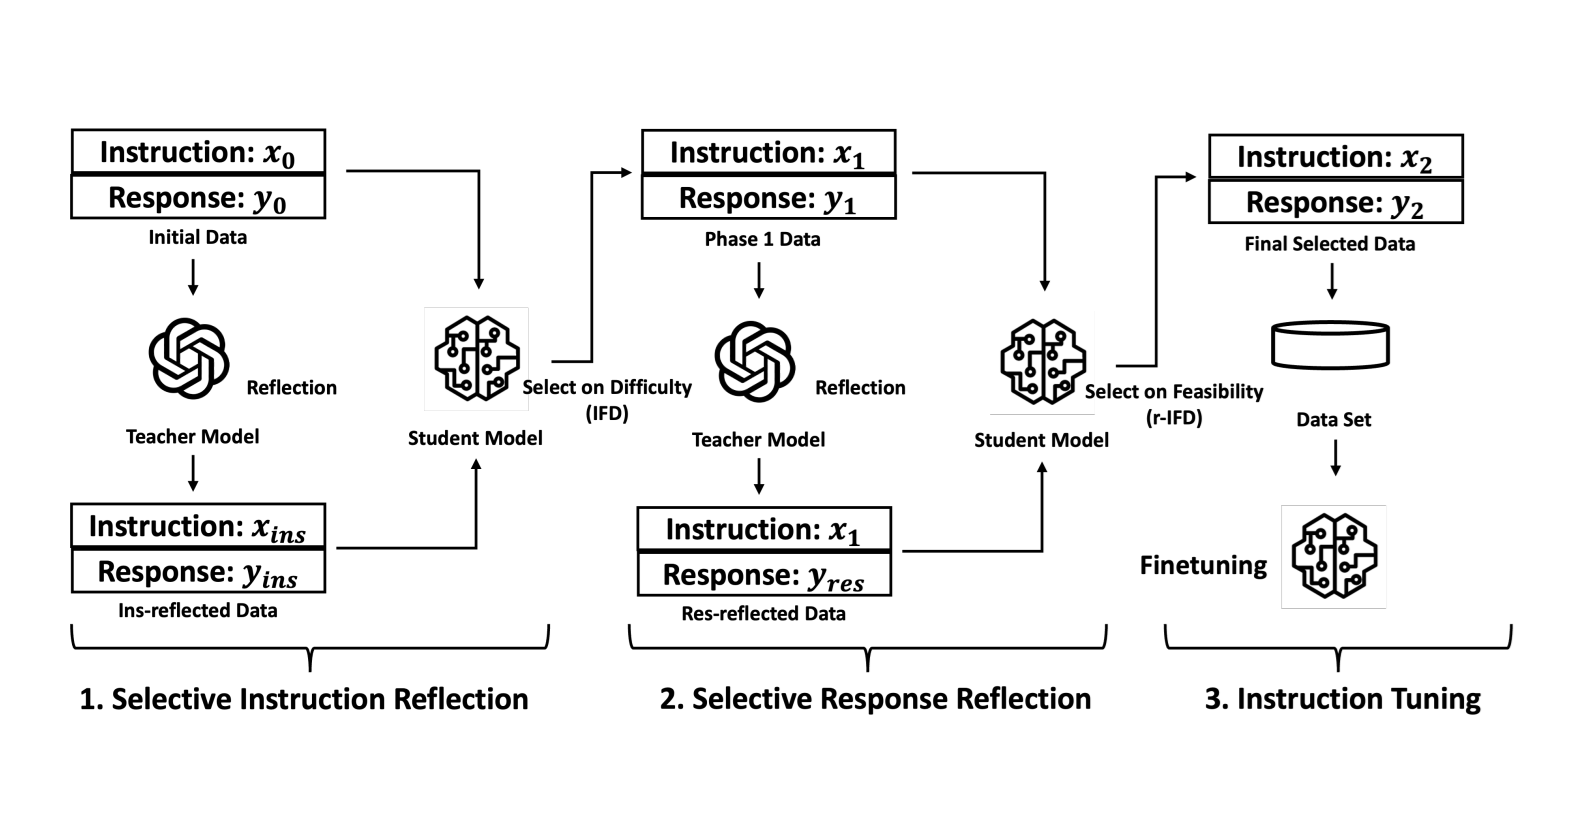
\includegraphics[width=0.8\textwidth]{Figs/Reflection tuning.png}
    \caption{Architettura del processo di \textit{Reflection Tuning}, con l'iterazione tra \textit{Teacher} e \textit{Student Model} nelle tre fasi di riflessione sulle istruzioni, riflessione sulla risposta e \textit{Instruction Tuning} finale sul dataset curato.}
    \label{fig:riflection_tuning}
\end{figure}

\subsection{Reflection Tuning come strategia di training}

Il \textbf{Reflection Tuning} rappresenta l'evoluzione metodologica che trasforma la capacità di riflessione da un comportamento emergente a un obiettivo di addestramento esplicito. A differenza del semplice \textit{Chain-of-Thought prompting} \cite{wei2022chain,kojima2022large}, in cui la riflessione è stimolata solo in fase di inferenza tramite istruzioni testuali (spesso con risultati variabili), il tuning modifica i pesi del modello affinché la riflessione diventi una competenza nativa, strutturale e predicibile. 

L'addestramento si basa su dataset di istruzioni arricchite che seguono una struttura a più stadi, formalizzabile come $\mathcal{D} = \{ (I, R, C, O)_i \}_{i=1}^N$. In questa formulazione, l'istruzione $I$ non porta direttamente all'output $O$, ma transita attraverso una riflessione iniziale $R$ e una fase di correzione $C$. L'inclusione deliberata di errori seguiti da rettifiche all'interno dei dati di addestramento è l'elemento cardine di questa strategia: insegnare al modello a riconoscere un proprio fallimento logico (\textit{error detection}) e a porvi rimedio in autonomia (\textit{error correction}) è ciò che distingue il Reflection Tuning dalle tecniche di fine-tuning convenzionali.



Un aspetto critico risiede nella gestione dei \textbf{token di delimitazione}, che fungono da barriere architettoniche tra il pensiero interno e la risposta esterna. Il modello viene addestrato a utilizzare tag specifici, come \texttt{<thought>}, \texttt{<analysis>} e \texttt{<correction>}, che permettono al sistema di isolare i flussi di elaborazione interna dall'interazione con l'utente, impedendo che i "dubbi" del modello sporchino la qualità del testo finale. 

Durante la fase di ottimizzazione, la funzione di perdita (\textit{loss function}) viene pesata strategicamente per incentivare non solo la correttezza della risposta $O$, ma soprattutto la precisione dei passaggi logici contenuti nella sezione di riflessione. Si assume infatti che la qualità dell'output sia una funzione diretta della qualità del pensiero intermedio. Questo approccio viene spesso potenziato tramite tecniche di \textbf{Reinforcement Learning from Human Feedback} (RLHF) \cite{ouyang2022training} o \textbf{Direct Preference Optimization} (DPO). In questi scenari, i modelli di ricompensa sono istruiti per premiare le tracce di riflessione che dimostrano un rigore metodologico elevato, una verifica accurata dei fatti e la capacità di scartare ipotesi errate, consolidando così un comportamento riflessivo che rende il modello non solo più accurato, ma anche più affidabile e interpretabile.

\subsection{Data recycling e auto-miglioramento}

La frontiera più avanzata del Reflection Tuning risiede nella risoluzione di un paradosso fondamentale: la scarsità di dati di addestramento di alta qualità che includano processi di riflessione espliciti e corretti. Poiché l'annotazione umana di "tracce di pensiero" è un processo estremamente costoso, lento e difficilmente scalabile per compiti di alta complessità scientifica o logica, la ricerca si è orientata verso tecniche di \textbf{Data Recycling} e cicli di \textbf{Auto-miglioramento} (\textit{Self-Improvement}). Queste metodologie permettono ai modelli di generare autonomamente il proprio materiale di studio, innescando un processo di apprendimento ricorsivo che non dipende esclusivamente da input esterni.

Il ciclo di auto-miglioramento si articola tipicamente attraverso un processo iterativo di esplorazione e raffinamento. Inizialmente, di fronte a un insieme di problemi complessi, il modello opera una \textit{generazione di tentativi multipli}, producendo diverse varianti di ragionamento e soluzione. Questo avviene variando la temperatura di campionamento per esplorare percorsi logici eterogenei. Successivamente, queste soluzioni vengono sottoposte a una fase di \textit{verifica tramite oracoli o modelli critici}. In domini deterministici come la matematica o la programmazione, la validazione è oggettiva e automatica, basata sull'accuratezza del risultato finale o sull'esecuzione di test unitari. In ambiti meno strutturati, interviene un modello "critico" (spesso un \textit{Teacher} di dimensioni superiori) con il compito di analizzare la coerenza formale della riflessione.



Il cuore pulsante di questa strategia è il \textit{re-training su dati filtrati}. Solo le traiettorie di pensiero che hanno condotto con successo alla soluzione corretta vengono integrate nel dataset di fine-tuning per il ciclo successivo. Questo meccanismo è alla base di algoritmi seminali come \textbf{STaR} (\textit{Self-Taught Reasoner}) \cite{zelikman2022star}, in cui il modello impara a razionalizzare a posteriori le risposte corrette che inizialmente aveva individuato in modo fortuito. In questo modo, le intuizioni statistiche si cristallizzano in regole logiche consolidate, permettendo al modello di "imparare a pensare" dai propri successi.

Tuttavia, l'autosufficienza del data recycling introduce sfide non trascurabili, in particolare il rischio di \textbf{bias amplification} e la cosiddetta "deriva semantica". Se il modello viene addestrato su riflessioni che contengono errori logici sottili o passaggi ridondanti non rilevati dai filtri, rischia di stabilizzare abitudini di ragionamento fallaci, seppur formalmente eleganti. Per mitigare tale deriva, le architetture più recenti adottano una \textbf{Knowledge Distillation incrociata} \cite{madaan2023self,shinn2023reflexion}. In questo scenario, la capacità di riflessione di modelli ultra-large (come i modelli della serie "o1" o DeepSeek-R1 \cite{deepseekr1_2025}) viene utilizzata per supervisionare e "pulire" i dati sintetici generati dai modelli più piccoli. 

Questo connubio tra auto-generazione e supervisione esterna garantisce che l'auto-miglioramento rimanga ancorato a standard di rigore logico elevati. Il Reflection Tuning cessa così di essere una semplice fase di addestramento statico per trasformarsi in un meccanismo di evoluzione cognitiva autonoma, dove lo Student non si limita a imitare il Teacher, ma utilizza gli strumenti logici acquisiti per esplorare e mappare autonomamente nuovi domini di conoscenza.

\section{LLM-as-a-Judge}
\label{sec:llm_judge}

La valutazione automatica delle risposte generate da modelli linguistici
rappresenta uno dei problemi aperti più rilevanti nell'ambito della
ricerca sugli LLM. Le metriche classiche basate sul confronto lessicale
--- come BLEU, ROUGE o METEOR --- si rivelano inadeguate per testi a
risposta aperta, in cui risposte semanticamente equivalenti possono
differire radicalmente nella formulazione superficiale. L'annotazione
umana, pur restando lo standard di riferimento, è costosa, lenta e
soggetta a variabilità inter-annotatore. Il paradigma
\textbf{LLM-as-a-Judge} \cite{zheng2023judging} propone una soluzione
intermedia: utilizzare un Large Language Model di elevata capacità come
giudice automatico che valuta la qualità delle risposte prodotte da
altri modelli.

L'idea fondamentale è che un LLM sufficientemente capace sia in grado
di apprezzare sfumature qualitative --- correttezza fattuale,
coerenza logica, chiarezza espositiva, utilità della risposta ---
in modo analogo a un valutatore umano esperto, ma a una frazione
del costo e del tempo. Il giudice riceve in input il testo della
domanda, la risposta (o le risposte) da valutare e un insieme di
criteri di giudizio specificati nel prompt di sistema. Produce in
output uno o più punteggi numerici su scale definite e,
facoltativamente, una motivazione testuale della valutazione.

La letteratura distingue tre configurazioni principali. Nel
\textbf{giudizio assoluto} (\textit{pointwise}), il giudice valuta
una singola risposta assegnando un punteggio su una scala discreta
(tipicamente 1--5 o 1--10) per ciascuna metrica di interesse; questa
modalità è adatta a valutare la qualità intrinseca di un modello
senza confronto diretto con altri. Nel \textbf{giudizio comparativo}
(\textit{pairwise}), vengono presentate al giudice le risposte di
due modelli diversi alla stessa domanda; il giudice deve determinare
quale sia preferibile, oppure dichiarare una parità. Questa modalità
riduce i bias di calibrazione assoluta e facilita il ranking relativo
tra sistemi. Infine, nel \textbf{giudizio su lista} (\textit{listwise}),
più risposte vengono ordinate simultaneamente, con il vantaggio di una
maggiore coerenza transitiva ma a costo di un prompt più complesso.

Il principale vantaggio dell'approccio LLM-as-a-Judge è la scalabilità:
permette di valutare migliaia di risposte in tempi ridotti e a costi
contenuti, rendendo possibili esperimenti di valutazione che sarebbero
proibitivi con annotatori umani. Studi empirici hanno mostrato
correlazioni elevate tra i giudizi prodotti da modelli come GPT-4
e le valutazioni umane su diversi benchmark \cite{zheng2023judging}.

Tuttavia, il paradigma presenta criticità note. Il \textbf{position
bias} è la tendenza del giudice a preferire sistematicamente la
risposta presentata per prima (o per ultima) indipendentemente dal
contenuto, mitigabile invertendo l'ordine delle risposte e
aggregando i giudizi. Il \textbf{verbosity bias} è la preferenza
per risposte più lunghe e articolate anche quando una risposta
concisa sarebbe più appropriata. Il \textbf{self-enhancement bias}
descrive la tendenza di un modello a favorire risposte stilisticamente
simili alle proprie, il che introduce un potenziale conflitto di
interessi quando il giudice coincide con il modello teacher usato
per generare i dati di training. Infine, i giudizi possono essere
sensibili alla formulazione del prompt: criteri espressi in modo
ambiguo portano a valutazioni inconsistenti anche a parità di risposta.
Nonostante questi limiti, l'LLM-as-a-Judge è oggi ampiamente adottato
come strumento di valutazione pratico nell'ambito della ricerca
sui modelli linguistici \cite{zheng2023judging}.
    \chapter{Applicazione}
\label{cap:3}

Questo capitolo descrive l'implementazione pratica del sistema di
confronto tra Reflection Tuning e Knowledge Distillation response-based
su un modello linguistico di piccola taglia. La pipeline è composta da
quattro fasi sequenziali: filtraggio e preparazione del dataset,
generazione del dataset di distillation tramite modello teacher,
fine-tuning QLoRA dei due modelli, e valutazione comparativa tramite
LLM-as-a-Judge. Il codice sorgente è organizzato in script Python
distinti, ciascuno corrispondente a una fase della pipeline.

% ------------------------------------------------------------
\section{Architettura della Pipeline}
\label{sec:pipeline_overview}
% ------------------------------------------------------------

La Figura~\ref{fig:pipeline} illustra la struttura complessiva del
sistema. La pipeline è progettata attorno a un principio di controllo
sperimentale rigoroso: le due strategie di addestramento devono
differire in una e una sola variabile --- la natura del dato di
training --- affinché i risultati finali siano attribuibili
esclusivamente a quella differenza e non a fattori confondenti come
la dimensione del dataset, la scelta del modello base o gli
iperparametri di ottimizzazione.

Il punto di ingresso comune è il corpus \textbf{OpenThoughts-114k}
\cite{openthoughts2024}, da cui vengono estratti 700 campioni di
training tramite una procedura di filtraggio basata sulla lunghezza
e qualità del ragionamento. Questi 700 campioni fungono da sorgente
per entrambi i rami della pipeline, garantendo che le domande a cui
i due modelli vengono esposti durante il training siano identiche.

La biforcazione avviene immediatamente dopo il filtraggio. Nel
\textbf{ramo sinistro} (Reflection Tuning), i campioni originali
vengono utilizzati direttamente: ciascuno contiene già una traccia
di ragionamento esplicita, prodotta da modelli di grandi dimensioni
al momento della creazione di OpenThoughts-114k, racchiusa in un
blocco \texttt{<thinking>}. Il modello student apprende a riprodurre
sia il ragionamento che la risposta finale, internalizzando una
struttura di pensiero a due stadi.

Nel \textbf{ramo destro} (Knowledge Distillation response-based),
le stesse 700 domande vengono inviate a \textbf{Gemini Flash} come
modello teacher tramite API. Il teacher produce per ciascuna una
risposta diretta e concisa, priva di ragionamento esplicito: l'obiettivo
del modello student è imitare lo stile e la correttezza di queste
risposte, secondo il paradigma del \emph{behavior cloning}. La
generazione del dataset di distillation costituisce quindi un passo
aggiuntivo rispetto al ramo Reflection, che introduce Gemini Flash
come fonte esterna di supervisione.

I due dataset risultanti --- Dataset Reflection e Dataset Distillation,
entrambi di 700 campioni --- vengono usati per addestrare separatamente
due istanze di \textbf{Llama 3.2 1B-Instruct} tramite \textbf{QLoRA}.
Il modello base, il metodo di quantizzazione (4-bit), il rango degli
adattatori LoRA ($r = 16$, $\alpha = 32$), il numero di epoche e il
learning rate sono identici per entrambi i training, in modo che la
procedura di ottimizzazione non introduca variabili aggiuntive nel
confronto.

Al termine del training, i due modelli addestrati convergono in
un'unica fase di \textbf{valutazione comparativa}: entrambi ricevono
le stesse 20 domande di test e le loro risposte vengono giudicate
da Gemini Flash secondo il paradigma LLM-as-a-Judge. Il giudice
valuta ogni coppia di risposte su tre metriche (Correctness, Reasoning
Quality, Clarity) e determina un vincitore per ciascuna domanda,
producendo i dati quantitativi analizzati nel capitolo successivo.

\begin{figure}[htbp]
  \centering
  \begin{tikzpicture}[
      box/.style={rectangle, draw, rounded corners,
                  minimum width=3.4cm, minimum height=1cm,
                  align=center, font=\small},
      arrow/.style={->, thick, >=stealth}
    ]
    \node[box] (ds)   at (3.5,  0)  {OpenThoughts-114k\\(114k sample)};
    \node[box] (filt) at (3.5, -2)  {Filtraggio e\\campionamento};
    \node[box] (refl) at (0,   -4)  {Dataset Reflection\\(700 sample)};
    \node[box] (teach)at (7,   -4)  {Teacher Gemini Flash\\(700 query)};
    \node[box] (dist) at (7,   -6)  {Dataset Distillation\\(700 sample)};
    \node[box] (tr1)  at (0,   -8)  {QLoRA Training\\Reflection};
    \node[box] (tr2)  at (7,   -8)  {QLoRA Training\\Distillation};
    \node[box] (eval) at (3.5, -10) {Evaluation\\LLM-as-a-Judge (Gemini Flash)};
    \draw[arrow] (ds)    -- (filt);
    \draw[arrow] (filt)  -- (refl);
    \draw[arrow] (filt)  -- (teach);
    \draw[arrow] (teach) -- (dist);
    \draw[arrow] (refl)  -- (tr1);
    \draw[arrow] (dist)  -- (tr2);
    \draw[arrow] (tr1)   -- (eval);
    \draw[arrow] (tr2)   -- (eval);
  \end{tikzpicture}
  \caption{Schema della pipeline sperimentale. Le frecce indicano il
    flusso dei dati. I due rami di training condividono lo stesso modello
    base (Llama~3.2~1B-Instruct) e gli stessi iperparametri.}
  \label{fig:pipeline}
\end{figure}

\FloatBarrier
% ------------------------------------------------------------
\section{Preparazione del Dataset}
\label{sec:step1}
% ------------------------------------------------------------

Il dataset di partenza è \textbf{OpenThoughts-114k}
\cite{openthoughts2024}, un corpus pubblico disponibile su
Hugging Face che raccoglie oltre 114\,000 conversazioni generate da
modelli di tipo \emph{chain-of-thought}. Ogni campione è strutturato
come una conversazione a due turni: una domanda dell'utente e una
risposta dell'assistente che include un blocco di ragionamento
delimitato dai tag \texttt{<|begin\_of\_thought|>} e
\texttt{<|end\_of\_thought|>}, seguito dalla soluzione finale.

\paragraph{Filtraggio.}
Lo script \texttt{prepare\_dataset.py} applica una pipeline di
filtraggio per selezionare i campioni di qualità sufficiente.
I campioni vengono accettati solo se soddisfano tutti i vincoli
definiti nella Tabella~\ref{tab:filtri}. I campioni validi vengono
rimescolati con seed fisso (\texttt{SEED = 42}) e suddivisi in
700 campioni di training e 80 campioni di valutazione.

\begin{table}[t]
  \centering
  \caption{Criteri di filtraggio applicati ai campioni di OpenThoughts-114k.}
  \label{tab:filtri}
  \small
  \renewcommand{\arraystretch}{1.3}
  \begin{tabular}{l l p{6cm}}
    \toprule
    \textbf{Parametro} & \textbf{Valore} & \textbf{Motivazione} \\
    \midrule
    \texttt{MIN\_THINKING\_LEN} & 300 car. &
      Esclude ragionamenti troppo superficiali \\
    \texttt{MAX\_THINKING\_LEN} & 6000 car. &
      Evita sequenze che superano il contesto del modello \\
    \texttt{MIN\_ANSWER\_LEN}   & 50 car. &
      Esclude risposte degeneri o incomplete \\
    Lunghezza minima thinking   & 50 parole &
      Filtra blocchi formalmente presenti ma privi di contenuto \\
    \bottomrule
  \end{tabular}
\end{table}

\paragraph{Formato di output.}
Ciascun campione viene riformattato nel formato conversazionale
atteso dal modello: il ragionamento estratto viene racchiuso nel
tag \texttt{<thinking>...</thinking>} e concatenato alla soluzione
finale, producendo la risposta dell'assistente che lo student dovrà
apprendere a generare.

\FloatBarrier
% ------------------------------------------------------------
\section{Generazione del Dataset di Distillation}
\label{sec:step1b}
% ------------------------------------------------------------

La preparazione del dataset di distillation segue due approcci
complementari. Il primo, implementato in
\texttt{build\_distillation\_dataset.py}, genera il dataset a partire
direttamente dal dataset reflection, rimuovendo i blocchi
\texttt{<thinking>} tramite espressione regolare e conservando solo
la risposta finale. Questo produce un dataset con le stesse domande
e risposte di base, con l'unica differenza della \emph{presenza o
assenza del ragionamento esplicito}.

Il primo approccio rimuove il blocco \texttt{<thinking>} tramite
espressione regolare, conservando solo il testo successivo al tag
di chiusura:

\begin{comment}
\begin{lstlisting}[language=Python, caption={Estrazione della risposta finale dal campione reflection.}]
match = re.search(r"</thinking>\s*\n*(.*)", content, re.DOTALL)
answer_only = match.group(1).strip()
\end{lstlisting}
\end{comment}

Il secondo approccio, implementato in
\texttt{generate\_teacher\_responses.py}, interroga \textbf{Gemini
Flash} (\texttt{gemini-2.5-flash}) come modello teacher: per
ciascuna delle 700 domande viene generata una risposta diretta senza
ragionamento esplicito, configurando uno scenario di \emph{knowledge
distillation response-based} in cui lo student impara a riprodurre
le risposte di un teacher più capace. Il sistema prompt fornito al
teacher specifica esplicitamente di non utilizzare tag XML di
reasoning:

\begin{lstlisting}[language=Python, caption={System prompt inviato a Gemini Flash come teacher.}, float=tbp]
SYSTEM_PROMPT = """You are a helpful and precise assistant.
Answer the user's question clearly and correctly.
Show your reasoning when solving problems, but be concise.
Do NOT use XML tags like <thinking> in your response."""
\end{lstlisting}

Per gestire i vincoli della quota gratuita dell'API (15 richieste al
minuto), lo script implementa un meccanismo di rate limiting con sleep
inter-chiamata di circa 4.3 secondi e un sistema di checkpoint ogni
10 chiamate, consentendo la ripresa in caso di interruzione. Il tempo
complessivo per la generazione delle 700 risposte è stato di circa
50 minuti.

\FloatBarrier
% ------------------------------------------------------------
\section{Fine-Tuning con QLoRA}
\label{sec:step2}
% ------------------------------------------------------------

Entrambi i modelli sono addestrati a partire da
\textbf{Llama~3.2~1B-Instruct} \cite{meta2024llama32}, nella variante
quantizzata a 4 bit (NF4) fornita da Unsloth. La quantizzazione tramite
\texttt{bitsandbytes} riduce l'utilizzo di memoria di circa il 75\%
rispetto alla precisione float16, rendendo il training fattibile su
GPU con 16\,GB di VRAM.

\subsection{Configurazione LoRA}

L'adattamento del modello è realizzato con \textbf{Low-Rank
Adaptation} \cite{hu2021lora} tramite la libreria PEFT. I parametri
adottati sono riportati nella Tabella~\ref{tab:lora}. I moduli target
coprono sia i layer di self-attention (\texttt{q\_proj},
\texttt{k\_proj}, \texttt{v\_proj}, \texttt{o\_proj}) sia i layer
feed-forward della MLP (\texttt{gate\_proj}, \texttt{up\_proj},
\texttt{down\_proj}), massimizzando la capacità di adattamento entro
i vincoli di memoria disponibile.

\begin{table}[t]
  \centering
  \caption{Iperparametri LoRA e di training condivisi tra i due esperimenti.}
  \label{tab:lora}
  \small
  \renewcommand{\arraystretch}{1.3}
  \begin{tabular}{l l l l l l}
    \toprule
    $r$ & $\alpha$ & Dropout & LR & Epoche & Batch eff. \\
    \midrule
    16 & 32 & 0.0 & $2{\times}10^{-4}$ & 3 & 8 \\
    \bottomrule
  \end{tabular}
\end{table}

\subsection{Procedura di training}

Gli iperparametri di training sono identici per entrambi i modelli
(Tabella~\ref{tab:lora}): learning rate $2 \times 10^{-4}$ con
ottimizzatore AdamW 8-bit, 3 epoche, batch size effettivo 8
(batch~2 con gradient accumulation~4), LR scheduler cosine con
warmup ratio 0.05, lunghezza massima della sequenza 2048 token e
seed 42. Questa scelta garantisce che qualunque differenza nelle
prestazioni finali sia attribuibile esclusivamente al formato dei
dati di addestramento.

Il modello di reflection è addestrato tramite \texttt{train\_reflection.py} con \\
\texttt{UnslothTrainer}, che applica ottimizzazioni specifiche per
sequenze lunghe con reasoning tag. Il modello di distillation è
addestrato tramite \texttt{train\_distillation.py} con
\texttt{SFTTrainer} della libreria TRL, con parametri equivalenti.
Al termine del training, le sole matrici LoRA vengono salvate come
adapter separati, con dimensione su disco dell'ordine di poche decine
di MB ciascuno.

\FloatBarrier
% ------------------------------------------------------------
\section{Valutazione Comparativa}
\label{sec:step3}
% ------------------------------------------------------------

\subsection{Procedura di inferenza}

Lo script \texttt{evaluate.py} carica entrambi i modelli sequenzialmente
e genera le risposte alle stesse 20 domande del test set con parametri
di decodifica identici:

\begin{lstlisting}[language=Python, caption={Parametri di generazione usati durante la valutazione.}, float=tbp]
outputs = model.generate(
    **inputs,
    max_new_tokens = 512,
    temperature    = 0.6,
    top_p          = 0.9,
    do_sample      = True,
    pad_token_id   = tokenizer.eos_token_id,
)
\end{lstlisting}

La temperatura $T = 0.6$ bilancia diversità e coerenza delle risposte;
il nucleus sampling con $p = 0.9$ tronca la distribuzione escludendo
i token meno probabili.

\subsection{LLM-as-a-Judge}

La valutazione delle risposte è delegata a \textbf{Gemini Flash}
in qualità di giudice automatico, secondo il paradigma
\emph{LLM-as-a-Judge} \cite{zheng2023judging}. Ad ogni coppia
di risposte viene sottoposto un prompt strutturato che richiede
al giudice di assegnare punteggi su tre dimensioni:

\begin{enumerate}
  \item \textbf{Correctness} (1--5): correttezza della risposta finale
  \item \textbf{Reasoning Quality} (1--5): qualità e coerenza del
    ragionamento mostrato
  \item \textbf{Clarity} (1--5): chiarezza e struttura espositiva
\end{enumerate}

e di indicare il vincitore complessivo tra i due modelli (A, B, o
parità). Il prompt sottoposto al giudice segue il template:

\begin{lstlisting}[language=Python, caption={Template del prompt per il giudice LLM.}, float=tbp]
JUDGE_PROMPT = """You are an expert evaluator comparing two AI
responses to a reasoning question.

Question: {question}
Model A (Distillation) response: {response_a}
Model B (Reflection)  response: {response_b}

Evaluate both on: CORRECTNESS, REASONING_QUALITY, CLARITY (1-5).
Then decide: which model is BETTER overall? (A, B, or TIE)

Respond ONLY in this JSON format:
{
  "model_a": {"correctness": 0, "reasoning_quality": 0, "clarity": 0},
  "model_b": {"correctness": 0, "reasoning_quality": 0, "clarity": 0},
  "winner": "A|B|TIE",
  "reasoning": "brief explanation"
}"""
\end{lstlisting}

Il giudice restituisce i risultati in formato JSON strutturato,
che viene parsato e salvato in \texttt{evaluation\_results.csv}.
Per contenere il numero di token inviati al giudice, le risposte
vengono troncate a 1000 caratteri. Il training è stato eseguito
interamente su \textbf{Google Colab} con GPU \textbf{NVIDIA Tesla T4}
(16\,GB VRAM) tramite la libreria Unsloth, che ottimizza le operazioni
di attenzione e il gradient checkpointing per sequenze lunghe.

    \chapter{Risultati}
\label{cap:4}

Questo capitolo presenta i risultati della valutazione comparativa tra
il modello addestrato con Reflection Tuning e quello addestrato con
Knowledge Distillation response-based. La valutazione è stata condotta
su un insieme di 20 domande di ragionamento matematico, giudicate
da Gemini Flash secondo il paradigma LLM-as-a-Judge descritto nel
capitolo precedente. Per ciascuna domanda sono stati raccolti punteggi
su tre metriche (Correctness, Reasoning Quality, Clarity) e un
giudizio complessivo di vittoria.


\section{Risultati Quantitativi}
\label{sec:risultati_quantitativi}

\subsection{Pipeline sperimentale e dati raccolti}
\label{subsec:pipeline_risultati}

Prima di presentare i risultati numerici è utile richiamare la
struttura della pipeline sperimentale, illustrata nella
Figura~\ref{fig:pipeline} del capitolo precedente.
Il punto di partenza è il dataset pubblico \textbf{OpenThoughts-114k},
composto da circa 114\,000 esempi di ragionamento generati da modelli
di grandi dimensioni. Da questo corpus sono stati estratti e filtrati
\textbf{700 campioni di training} e \textbf{80 campioni di valutazione},
selezionando conversazioni con tracce di ragionamento di lunghezza e
qualità sufficienti a garantire la supervisione del modello.

A partire dagli stessi 700 campioni, la pipeline si biforca in due
rami paralleli e simmetrici, ciascuno destinato ad addestrare una
versione distinta di Llama~3.2~1B-Instruct. Nel \textbf{ramo
Reflection}, le 700 conversazioni originali --- già dotate di un
blocco \texttt{<thinking>} con il ragionamento esplicito generato
da modelli di grandi dimensioni --- vengono utilizzate direttamente
come target di fine-tuning: lo student impara a produrre, per ogni
domanda, sia la traccia di ragionamento sia la risposta finale,
replicando la struttura a due stadi del dato originale. Nel \textbf{ramo
Distillation}, le stesse 700 domande vengono sottoposte a Gemini
Flash (il modello \emph{teacher}), che restituisce per ciascuna una
risposta diretta e concisa, priva di ragionamento esplicito: questo
secondo dataset di 700 coppie domanda--risposta viene usato per
addestrare lo student secondo il paradigma del \emph{behavior cloning},
in cui l'obiettivo è imitare lo stile e la correttezza del teacher.

Entrambi i modelli vengono addestrati con \textbf{QLoRA} (rango
$r = 16$, $\alpha = 32$, quantizzazione 4-bit) per lo stesso numero
di epoche e con gli stessi iperparametri, in modo da rendere il
confronto finale attribuibile esclusivamente alla natura del dato
di training e non a differenze nella procedura di ottimizzazione.
Al termine del training, i due modelli vengono valutati su un test
set comune di \textbf{20 domande di ragionamento matematico},
somministrate a entrambi nello stesso ordine. Le risposte vengono
giudicate da Gemini Flash secondo il paradigma \textbf{LLM-as-a-Judge}
\cite{zheng2023judging}: per ogni domanda il giudice assegna un
punteggio da 1 a 5 su tre metriche (\emph{Correctness},
\emph{Reasoning Quality}, \emph{Clarity}) e un giudizio complessivo
di vittoria. La domanda Q18 ha prodotto un errore API durante la
fase di evaluation e non è inclusa nel calcolo delle medie ($n = 19$).

La Tabella~\ref{tab:medie} riassume i punteggi medi per metrica;
la Tabella~\ref{tab:winner} riporta la distribuzione dei giudizi
complessivi; la Tabella~\ref{tab:perdomanda} mostra il dettaglio
per ciascuna delle 20 domande.

\begin{table}[tbp]
  \centering
  \caption{Punteggi medi per metrica (scala 1--5, $n = 19$).}
  \label{tab:medie}
  \small
  \renewcommand{\arraystretch}{1.4}
  \begin{tabular}{lcccc}
    \toprule
    \textbf{Metrica} &
    \textbf{Distillation} &
    \textbf{Reflection} &
    \textbf{$\Delta$ (R $-$ D)} \\
    \midrule
    Correctness       & 3.89 & 2.74 & $-$1.16 \\
    Reasoning Quality & 3.74 & 3.05 & $-$0.68 \\
    Clarity           & 4.11 & 2.42 & $-$1.68 \\
    \midrule
    \textbf{Media complessiva} & \textbf{3.91} & \textbf{2.74} & $-$\textbf{1.17} \\
    \bottomrule
  \end{tabular}
\end{table}

\begin{table}[tbp]
  \centering
  \caption{Distribuzione dei giudizi di vittoria su 19 domande valide.}
  \label{tab:winner}
  \small
  \renewcommand{\arraystretch}{1.4}
  \begin{tabular}{lcc}
    \toprule
    \textbf{Esito} & \textbf{Conteggio} & \textbf{Percentuale} \\
    \midrule
    Distillation (A) & 14 & 73.7\% \\
    Reflection (B)   &  5 & 26.3\% \\
    Parità (TIE)     &  0 &  0.0\% \\
    \bottomrule
  \end{tabular}
\end{table}

Il modello di distillation ottiene punteggi superiori in tutte e tre
le dimensioni valutate e vince in 14 domande su 19 (73.7\%), senza
alcun pareggio. Il divario più marcato riguarda la metrica
\emph{Clarity} ($\Delta = -1.68$); il divario minore si osserva sulla
\emph{Reasoning Quality} ($\Delta = -0.68$), suggerendo che il modello
reflection, pur perdendo complessivamente, riesce in alcuni casi a
produrre sequenze di ragionamento di qualità comparabile.

La Tabella~\ref{tab:perdomanda} riporta il dettaglio per domanda.

\begin{table}[tbp]
  \centering
  \caption{Punteggi per domanda. C = Correctness, Q = Reasoning Quality,
    Cl = Clarity. Con * la domanda Q18 per cui il giudice ha restituito
    un errore API.}
  \label{tab:perdomanda}
  \resizebox{\textwidth}{!}{%
  \renewcommand{\arraystretch}{1.2}
  \begin{tabular}{clccccccl}
    \toprule
    \textbf{\#} & \textbf{Domanda (sintesi)} &
    \textbf{D\,C} & \textbf{D\,Q} & \textbf{D\,Cl} &
    \textbf{R\,C} & \textbf{R\,Q} & \textbf{R\,Cl} &
    \textbf{Vincitore} \\
    \midrule
    1  & Resto su acquisto mele        & 5 & 2 & 1 & 5 & 4 & 3 & Reflection \\
    2  & Velocità media treno          & 1 & 1 & 2 & 5 & 5 & 5 & Reflection \\
    3  & Dimensioni rettangolo         & 1 & 1 & 3 & 5 & 5 & 5 & Reflection \\
    4  & Numero ragazzi in classe      & 5 & 5 & 5 & 5 & 3 & 2 & Distillation \\
    5  & Lavoratori e giorni           & 5 & 5 & 5 & 1 & 1 & 1 & Distillation \\
    6  & Prezzo originale camicia      & 5 & 4 & 3 & 1 & 2 & 2 & Distillation \\
    7  & Equazione $x + 3 = 10$        & 5 & 5 & 5 & 4 & 5 & 2 & Distillation \\
    8  & Distanza automobile           & 5 & 5 & 5 & 1 & 2 & 2 & Distillation \\
    9  & Somma angoli pentagono        & 5 & 5 & 5 & 5 & 3 & 2 & Distillation \\
    10 & Divisibile per 4 e 6          & 5 & 4 & 4 & 1 & 2 & 3 & Distillation \\
    11 & Probabilità pallina rossa     & 1 & 2 & 3 & 2 & 4 & 2 & Reflection \\
    12 & Giorno della settimana        & 1 & 1 & 4 & 2 & 4 & 3 & Reflection \\
    13 & Altezza scala appoggiata      & 5 & 5 & 5 & 1 & 2 & 1 & Distillation \\
    14 & Equazione $2(x+4) = 3x-1$     & 5 & 5 & 5 & 1 & 2 & 2 & Distillation \\
    15 & Farina per biscotti           & 5 & 4 & 4 & 1 & 3 & 2 & Distillation \\
    16 & 15\% di 240                   & 1 & 3 & 4 & 1 & 2 & 2 & Distillation \\
    17 & Perimetro quadrato            & 5 & 5 & 5 & 3 & 3 & 2 & Distillation \\
    18 & Vasca con rubinetto*          & {--} & {--} & {--} & {--} & {--} & {--} & Errore API \\
    19 & Sequenza geometrica           & 4 & 4 & 5 & 3 & 2 & 2 & Distillation \\
    20 & Calcolo $f(2)$ con polinomio  & 5 & 5 & 5 & 5 & 4 & 3 & Distillation \\
    \midrule
    \multicolumn{2}{l}{\textbf{Media}} &
    3.89 & 3.74 & 4.11 & 2.74 & 3.05 & 2.42 & \\
    \bottomrule
  \end{tabular}}
\end{table}

\FloatBarrier
% ------------------------------------------------------------
\section{Analisi dei Risultati}
\label{sec:analisi}
% ------------------------------------------------------------

\subsection{Casi in cui la distillation prevale}

Il modello di distillation vince in 14 domande, con un pattern
abbastanza netto: nelle domande in cui la risposta richiede un calcolo
diretto o l'applicazione di una formula elementare (Q4, Q5, Q8, Q9,
Q13, Q14, Q15, Q17), il modello produce risposte corrette, concise
e ben strutturate, che il giudice valuta con il massimo punteggio
su tutte e tre le metriche.

In questi casi il modello reflection produce invece risposte
spesso errate (Correctness $= 1$) o incomplete, con punteggi di
Clarity molto bassi (frequentemente 1 o 2). Questo suggerisce che
il modello da 1B parametri, addestrato su soli 700 campioni, non
ha appreso in modo stabile il formato \texttt{<thinking>}, generando
in molti casi output mal strutturati in cui il ragionamento interno
non converge alla risposta corretta.

Un caso esemplificativo è la domanda Q5 (``Se 5 operai completano
un lavoro in 8 giorni, quanti giorni occorrono a 10 operai?''):
il modello di distillation produce la risposta corretta (4 giorni)
con un ragionamento lineare e punteggi massimi, mentre il modello
reflection ottiene il punteggio minimo su tutte le metriche,
indicando un output probabilmente incompleto o incoerente.

\subsection{Casi in cui la reflection prevale}

Il modello reflection vince in 5 domande (Q1, Q2, Q3, Q11, Q12).
L'analisi di questi casi rivela due sottotipi distinti:

\paragraph{Errori del modello di distillation (Q2, Q3, Q10, Q12).}
In questi casi il modello di distillation produce una risposta errata
(Correctness $= 1$), mentre il modello reflection riesce a fornire
la risposta corretta, probabilmente grazie al ragionamento esplicito
nel blocco \texttt{<thinking>} che funge da scaffolding per il
calcolo. La domanda Q2 (velocità media del treno) è un esempio
rappresentativo: il modello di distillation compie un errore
aritmetico elementare e produce una risposta sbagliata, mentre il
modello reflection percorre correttamente i passaggi di calcolo nel
blocco di thinking e giunge alla risposta esatta.

\paragraph{Parità sulla correttezza, vantaggio sulla qualità del ragionamento (Q1).}
Nella domanda Q1 entrambi i modelli rispondono correttamente, ma
il modello di distillation produce una risposta caratterizzata da
forte ridondanza (lo stesso ragionamento viene ripetuto più volte),
che il giudice penalizza con Clarity $= 1$ e Reasoning Quality $= 2$.
Il modello reflection, pur con Clarity inferiore alla media,
presenta un processo di ragionamento più coerente e viene giudicato
superiore.

\paragraph{Problemi con ragionamento non deterministico (Q11, Q12).}
Per le domande sulla probabilità e sul calendario, entrambi i modelli
mostrano difficoltà (Correctness $\leq 2$ per entrambi), ma il modello
reflection ottiene punteggi di Reasoning Quality superiori (4 vs.\ 1--2),
indicando che anche in presenza di una risposta finale errata il
blocco di thinking mostra un tentativo di ragionamento più articolato.

\subsection{Analisi per tipologia di domanda}

I risultati mostrano una dipendenza dalla tipologia del problema:

\begin{itemize}
  \item \textbf{Aritmetica diretta e algebra elementare} (Q4, Q7, Q8,
    Q9, Q14, Q17, Q20): distillation domina con punteggi massimi.
    Il modello ha appreso efficacemente lo stile conciso di Gemini Flash
    per problemi a soluzione rapida.

  \item \textbf{Problemi con struttura intermedia} (Q2, Q3, Q6, Q13,
    Q15): risultati misti. Distillation vince nella maggioranza, ma
    commette errori su problemi che richiedono più passaggi (Q2, Q3).

  \item \textbf{Ragionamento combinatorio e probabilistico} (Q11, Q12):
    entrambi i modelli faticano, ma reflection mostra un tentativo
    di ragionamento più esplicito, sebbene non sempre corretto.
\end{itemize}

\FloatBarrier
% ------------------------------------------------------------
\section{Discussione}
\label{sec:discussione}
% ------------------------------------------------------------

\subsection{Interpretazione generale}

I risultati indicano che, nelle condizioni sperimentali di questo
lavoro, il modello addestrato con knowledge distillation response-based
da Gemini Flash supera il modello addestrato con reflection tuning
su quasi tutte le metriche e tipologie di domanda. Tuttavia,
prima di trarre conclusioni generali, è necessario contestualizzare
questi risultati rispetto ai vincoli del setup sperimentale.

Il vantaggio della distillation è in larga misura attribuibile alla
\textbf{qualità assoluta delle risposte del teacher}. Gemini Flash
è un modello con capacità significativamente superiori a Llama
3.2 1B, e le sue risposte alle domande di matematica elementare sono
tendenzialmente corrette, concise e ben strutturate. Il modello
student ha potuto imitare questo stile in modo efficace, raggiungendo
punteggi di Clarity molto alti (media 4.11).

Al contrario, il dataset di reflection tuning contiene catene di
pensiero generate da modelli di reasoning di grandi dimensioni,
il cui stile verboso e articolato risulta difficile da replicare
per un modello da 1B parametri con training limitato. Il risultato
è che il modello reflection produce frequentemente output mal
strutturati o incompleti, penalizzati su tutte le metriche.

\subsection{Il ruolo del reasoning esplicito}

Nonostante i risultati complessivamente negativi per il reflection
tuning, i cinque casi in cui questo approccio prevale offrono
un'indicazione interessante: il ragionamento esplicito nel blocco
\texttt{<thinking>} sembra fungere da meccanismo di auto-correzione
su problemi che richiedono più passaggi di calcolo. Quando il modello
di distillation fallisce su questi problemi (Q2, Q3), il modello
reflection riesce a trovare la soluzione corretta percorrendo
esplicitamente i passaggi intermedi.

Questo è coerente con la letteratura sul \emph{chain-of-thought
prompting} \cite{wei2022chain}, che documenta come il
ragionamento esplicito migliori le prestazioni sui problemi che
richiedono composizione di passi. Il limite osservato è che un
modello da 1B parametri non dispone della capacità sufficiente
a mantenere un ragionamento coerente per l'intera durata del blocco
di thinking, degenerando spesso in ripetizioni o divergenze logiche.

\subsection{Confronto con la letteratura}

I risultati sono coerenti con le osservazioni riportate in lavori
recenti sul \emph{small language model fine-tuning}. Lavori come
Alpaca \cite{taori2023alpaca} e Vicuna \cite{chiang2023vicuna}
hanno mostrato che modelli di piccola taglia beneficiano
significativamente dall'imitazione di risposte di teacher più
capaci, anche in assenza di soft targets. D'altra parte, la
superiorità del reflection tuning su modelli di scala maggiore
è documentata in lavori come DeepSeek-R1 \cite{deepseekr1_2025}
e OpenAI o1, che adottano architetture e dataset di training
molto più grandi di quelli disponibili in questo esperimento.

La differenza tra i risultati di questo lavoro e quelli della
letteratura sul reasoning tuning è quindi spiegabile principalmente
dalla scala: con modelli da 7B parametri o superiori e dataset
di training nell'ordine delle decine di migliaia di campioni,
il reflection tuning mostra vantaggi consistenti che a scala 1B
non emergono in modo stabile.

\subsection{Limiti dell'interpretazione}

Alcune cautele sono necessarie nell'interpretare questi risultati:

\begin{itemize}
  \item Il test set è composto da sole 19 domande valide, il che
    non consente di trarre conclusioni statisticamente significative.
    La distribuzione 14--5 osservata potrebbe non essere stabile
    su un insieme di valutazione più ampio.

  \item Il giudice automatico (Gemini Flash) è lo stesso modello
    utilizzato per generare il dataset di distillation. Non si può
    escludere un bias stilistico che favorisce risposte simili a
    quelle che il giudice produce autonomamente.

  \item Le 20 domande coprono esclusivamente matematica e logica
    elementare. I risultati potrebbero differire su domini diversi,
    in particolare su problemi che richiedono ragionamento multi-passo
    più complesso, dove il blocco \texttt{<thinking>} potrebbe
    offrire un vantaggio maggiore.
\end{itemize}


    \chapter{Conclusioni}
\label{cap:5}

Questo lavoro ha confrontato due strategie di fine-tuning per il
trasferimento di capacità di ragionamento a modelli linguistici di
piccola taglia: il Reflection Tuning, basato sull'addestramento su
sequenze con ragionamento esplicito, e la Knowledge Distillation
response-based, basata sull'imitazione delle risposte di un modello
teacher più capace.

A partire dal dataset pubblico OpenThoughts-114k, sono stati estratti
700 campioni di training e 80 di valutazione. Il dataset di
distillation è stato generato interrogando Gemini Flash come teacher
su ciascuna delle 700 domande. I due dataset sono stati usati per
addestrare separatamente due versioni di Llama~3.2~1B-Instruct tramite
QLoRA, mantenendo identici tutti gli iperparametri. La valutazione
finale su 20 domande di ragionamento matematico è stata condotta con
Gemini Flash secondo il paradigma LLM-as-a-Judge \cite{zheng2023judging}.

I risultati mostrano una netta prevalenza del modello addestrato con
knowledge distillation: su 19 domande valide, il modello di
distillation vince in 14 casi (73.7\%), con punteggi medi superiori
in tutte e tre le metriche (Correctness 3.89 vs.\ 2.74, Reasoning
Quality 3.74 vs.\ 3.05, Clarity 4.11 vs.\ 2.42). Il vantaggio è
particolarmente marcato sulla Clarity ($\Delta = -1.68$), mentre si
riduce sulla Reasoning Quality ($\Delta = -0.68$), l'unica dimensione
in cui il modello reflection mostra risultati competitivi: nei cinque
casi in cui prevale, il blocco \texttt{<thinking>} sembra fungere da
meccanismo di auto-correzione su problemi multi-passo. Questi risultati
sono coerenti con la letteratura: a 1B parametri, l'imitazione diretta
di un teacher capace produce un comportamento più stabile rispetto
all'apprendimento di strutture di ragionamento complesse, che richiedono
scala e dati significativamente maggiori \cite{taori2023alpaca,wei2022chain}.

I risultati devono essere letti considerando i vincoli pratici
dell'intero lavoro. L'addestramento su Google Colab con GPU Tesla T4
gratuita ha imposto un tetto alla dimensione del modello utilizzabile:
architetture di scala superiore, su cui i vantaggi del reflection
tuning sono documentati in letteratura \cite{deepseekr1_2025}, erano
fuori portata. Il dataset di 700 campioni è stato vincolato dalla quota
gratuita dell'API Gemini (15 richieste/minuto) e dai limiti di sessione
di Colab; la valutazione su 20 domande consente di osservare tendenze
qualitative ma non conclusioni statisticamente significative. Va inoltre
precisato che la knowledge distillation implementata è di tipo
response-based --- lo student impara a imitare le risposte finali ---
e non incorpora i soft targets della formulazione classica
\cite{hinton2015distilling}, inaccessibili tramite API commerciali.
Il confronto è quindi più precisamente descritto come \emph{SFT su
dati con ragionamento esplicito} vs.\ \emph{SFT su risposte di un
modello capace}. Infine, il giudice automatico (Gemini Flash) coincide
con il teacher del modello di distillation, introducendo un potenziale
bias stilistico non quantificabile in assenza di valutatori indipendenti.

Per approfondimenti futuri, replicare l'esperimento con modelli di
scala maggiore (7B parametri o superiori) permetterebbe di verificare
se il vantaggio del reflection tuning emerge in modo più consistente.
Ampliare il dataset e il test set --- includendo benchmark standardizzati
come GSM8K \cite{cobbe2021gsm8k} o MATH \cite{hendrycks2021math} ---
consentirebbe una valutazione più robusta e confrontabile con la
letteratura. Sarebbe inoltre interessante esplorare un approccio ibrido
a due stadi: prima il teacher per acquisire correttezza di base, poi
dati con ragionamento esplicito per sviluppare capacità di auto-correzione.

Nonostante i vincoli, questo lavoro dimostra la fattibilità di una
pipeline completa di fine-tuning comparativo su hardware consumer-grade.
Il risultato principale --- la superiorità della distillation
response-based nelle condizioni adottate --- non confuta il reflection
tuning, ma indica che scala del modello e dimensione del dataset sono
fattori determinanti per sfruttare efficacemente il ragionamento
esplicito nel training. In altre parole, insegnare a un modello piccolo
a \emph{pensare ad alta voce} richiede che quel modello abbia già la
capacità di pensare: a 1B parametri, con 700 esempi, quella capacità
non è ancora sufficiente a tradursi in un vantaggio misurabile.

    \bibliographystyle{apalike}
    
    
    %\bibliographystyle{plainnat} % use this to have URLs listed in References
    %\cleardoublepage
    \bibliography{References/references} 
    \pagestyle{empty}% Path to your References.bib file
    \input{Chapters/6_ringraziamenti}
\end{document}